\documentclass[11pt]{amsart}

\usepackage{macros}

\spacing{1.25}

\addbibresource{references.bib}

\author{Natalie M. Paquette}
\address{Institute for Advanced Study, School of Natural Sciences, Princeton NJ, 08540, USA}
\address{Department of Physics, University of Washington, Seattle, WA, 98195-1560, USA}
\email{npaquett@uw.edu}
\author{Brian R. Williams}
\address{School of Mathematics, University of Edinburgh, Edinburgh, UK}
\email{brianwilliams.math@gmail.com}

\date{\today}
\title{Koszul duality in quantum field theory}

\def\brian#1{{\textcolor{blue!65!red}{BRW: {#1}}}}
\def\natalie#1{{\textcolor{green!65!black}{NMP: {#1}}}}

\begin{document}
\maketitle

\begin{abstract}
In this article, we introduce basic aspects of the algebraic notion of Koszul duality for a physics audience. We then review its appearance in the physical problem of coupling QFTs to topological line defects, and illustrate the concept with some examples drawn from twists of various simple supersymmetric theories. Though much of the content of this article is well-known to experts, the presentation and examples have not, to our knowledge, appeared in the literature before. Our aim is to provide an elementary introduction for those interested in the appearance of Koszul duality in supersymmetric gauge theories with line defects and, ultimately, its generalizations to higher-dimensional defects and twisted holography. 
\end{abstract}


\section{Introduction}
\natalie{preview quantum mechanical deformations of algebras}

\natalie{geometric quantization on the bubble}

\subsection*{Notations}

Cohomological shift. 



\section{A short review of Koszul duality} 

%sym and alt
%maybe a few words about mapping of modules btw derived categories? how does this relate to the line picture?
%CE(g) and U(g)
We begin by providing a basic introduction to Koszul duality for associative algebras, emphasizing the most simple algebraic examples. Since our aim is expository, we will omit many important references and generalizations. For a more exhaustive and general introduction to Koszul duality in mathematics see, for example, \cite{LV}.  \natalie{other canonical references?}

Let $\cA$ be an associative algebra.
We will often work in the more general situation where $\cA$ is a differentially graded (dg) algebra. A dg-algebra is $\ZZ$-graded algebra equipped with a square-zero, degree one operator $\d \colon \cA \to \cA[1]$ such that 
\[
\d (a \cdot b) = (\d a) \cdot b + (-1)^{|a|} a \cdot (\d b) 
\]
where $|a|$ denotes the degree of the element $a$. In physical contexts, one should think about $\cA$ as being the algebra of operators of a quantum mechanical system, and $\d$ may be a BRST operator or a square-zero supercharge, with the operators graded by ghost number or fermion number respectively \footnote{In many physical and mathematical contexts, we only require a $\ZZ/2\ZZ$ grading, e.g. fermion parity, but we will restrict to the $\ZZ$-graded case for now.}.
If we forget the product then $(\cA, \d)$ has the structure of a cochain complex. 
We work over the complex numbers $\CC$ so all products and maps are required to be $\CC$-linear. 

The notion of an $\cA$-module will also be taken in the dg sense. A dg $\cA$-module is a cochain complex $(M, \d_M)$ together with an $\cA$-module structure on $M$ which preserves the gradings and both the differentials $\d, \d_M$. 
When $\d_M = 0$ this returns the usual notion of an $\cA$-module. 
Unless there is room for confusion, when we speak of algebras and modules we are referring to the dg version.

\brian{what to say about $M$, defects?}
 
A map of algebras $f \colon \cA \to \cB$ is a map of cochain complexes which also preserves the associative products.
Notice that $f$ endows $\cB$ with the structure of a dg $\cA$-module by the formula $a \cdot b := f(a) \cdot b$, for $a \in \cA$ and $b \in \cB$, where the on the right hand side we use the associative product on $\cB$.  \natalie{the RHS is the *definition* of the LHS right?}

Similarly one can define a map of modules for a fixed algebra $\cA$.  All $\cA$-modules combine to form a category that we denote $\cA-\mod$.
This category has the structure of a dg category, which means its set of morphisms is equipped with the structure of a cochain complex (roughly, the space of Homs between any two fixed modules is graded and equipped with a nilpotent differential). 

Given $M,N \in \cA-\mod$ we denote by $\RHom_\cA(M,N)$ \natalie{add a footnote here about what the R in RHom means} the dg vector space of homomorphisms in the {\em derived category}. 
We will not use the full technology of derived categories in this note, but we remark on some important features to give the reader some intuition. 
The $i$th cohomology of the complex $\RHom_{\cA} (M,N)$ comprises the Ext groups ${\rm Ext}^i_{\cA}(M,N)$. 
For all $M,N$ the group ${\rm Ext}^0_{\cA}(M,N)$ agrees with the naive space of $\cA$-linear homomorphisms $M \to N$. 
The space ${\rm Ext}^1_{\cA}(M,N)$ is also relatively easy to understand: it is the space of equivalence classes of short exact sequences of $\cA$-modules of the form
\[
0 \to N \to E \to M \to 0 .
\]
\natalie{how are the equivalence classes defined?}

When $M = N$ the dg vector space $\RHom_\cA(M,M)$ acquires the structure of a dg algebra.
The zeroth cohomology agrees with the algebra of $\cA$-linear endomorphisms ${\rm End}_{\cA}(M)$.  
In general, to compute the space of derived homomorphisms one needs to first \textit{freely resolve} the module $M$, and we will see an example shortly.

A particularly important structure on an algebra will be that of an augmentation. 
An {\em augmentation} on a dg algebra $\cA$ is a map of dg algebras 
\[
\ep \colon \cA \to \CC 
\]
meaning that $\ep (a b) = \ep(a) \ep(b)$ and $\ep (\d a) = 0$. This augmentation may have a nontrivial kernel, which acts trivially on $\CC$. 
In other words, an augmentation defines the data of an $\cA$-module structure on the one-dimensional module. A choice of augmentation corresponds physically to a choice of vacuum. In our examples in this note, the augmentation is unique; we plan to expand on explicit examples with vacuum degeneracy (both massive vacua and moduli spaces of vacua) in subsequent work. \natalie{right? if we are feeling too lazy then we can remove this :)}
When we want to stress this interpretation of an augmentation, we denote the one-dimensional module by~$\CC_\ep$.


The Koszul dual of a dg algebra $\cA$ is the dg algebra
\[
\cA^! \define \RHom_\cA(\CC_\ep,\CC_\ep) .
\] 
Notice that the Koszul dual of $\cA$ is defined with respect to an augmentation $\ep$, though when the augmentation is understood we will omit it from the notation. Roughly speaking, this denotes that the Koszul dual algebra is the space of symmetries of the trivial module that commute with $\cA$. Further, notice that even if a dg-algebra $\cA$ is an ordinary associative algebra with trivial differential, its Koszul dual will be a complex with support in cohomological degrees $\geq 1$. 

One can show that the Koszul dual of $\cA^{!}$ is $\cA$ \natalie{is this easy to see without using anything too derived? if so, we should say a bit more}:
\[
\cA = \RHom_{\cA^!}(\CC_\ep, \CC_\ep).
\]
In other words, with the choice of augmentation, $\CC_\ep$ is simultaneously a module for $\cA, \cA^!$, and these algebras have commuting actions on $\CC_\ep$.

\natalie{please check and see if you agree with the discussion below. Should we say anything more/different about modules?}

Throughout this note, we will focus on the computation of Koszul dual algebras. However, we note that modules for these algebras are also of physical and mathematical interest. In fact, the derived categories of dg-modules of Koszul dual algebras are equivalent \footnote{More generally, certain triangulated subcategories may be equivalent \natalie{refs? I actually don't understand this subtlety in physical or math examples myself... plus, physicists mostly don't understand triangulated categories...}.}. We can denote this category $\cC \simeq \cA-\mod \simeq \cA^!-\mod$. We will make a few remarks on dg-modules throughout the note to orient the reader. 

\natalie{check that later in the paper we say something about the physical picture as e.g. defects on which lines can end, perhaps relation to topological boundary conditions?}

\subsection{Free field example} 

To illustrate the abstract considerations above, we present a short computation of the Koszul dual of the free symmetric algebra on a single (bosonic) generator, $\cA = \CC[x]$. 
The augmentation $\ep$ is the obvious one which sends a polynomial to its constant coefficient. 

The resulting one-dimensional module $\CC_{\ep}$ is not free (i.e. it does not admit a presentation in terms of linearly independent basis elements) as a $\CC[x]$-module, so, in order to make efficient computations, we need to find a cochain complex of free modules which resolves it. (The prototypical example of a free module is a vector space). 

\natalie{please feel free to edit or expand on this}Note that using the technique of resolving a module into a chain complex  is not unheard-of in physics: indeed, BRST quantization for some gauge group $G$ involves making a so-called projective resolution of the space of $G$-invariant local operators. The corresponding complex introduces fields of nonzero ghost number and a BRST differential. The cohomology of the BRST complex reproduces $G$-invariant local operators concentrated in degree 0 (the physical observables), and cohomologies in higher ghost number vanish. Similarly, BV quantization provides a resolution of the critical locus, i.e. solutions of the Euler-Lagrange equations, of a Lagrangian quantum field theory using antifields and antighosts. The resulting complex is called the Koszul-Tate complex. In general, a resolution of some module is simply a chain complex whose cohomology reproduces the original module; in homological algebra, this allows for efficient representation of invariant submodules or quotient modules using the tools of (nicely behaved) free or projective (etc.) modules. A bit more stringently, we require that there is a chain map from the original module to its resolution that induces an isomorphism in cohomology. The resulting chain map is called a quasi-isomorphism. Different quasi-isomorphic representations of the same module can have useful physical interpretations, even though the physical observables of interest involve the passage back to cohomology. To take a particularly simple instance, Yang-Mills theory can be quantized using the minimal BRST complex or using the full machinery of the BV-BRST complex, which are quasi-isomorphic complexes.\footnote{\natalie{do we want to say anything here about a "minimal complex" and Koszul duality? or elsewhere?}}.\natalie{nice physics example of useful different quasi-iso'c representations? an example from a physical duality?} 
\natalie{Do we want to add anything about free resolutions as solutions to PDEs as a more down-to-earth example here?}

A natural choice for a free resolution in this example is the so-called ``Koszul complex'', a progenitor of the Koszul-Tate complex in BV-quantization, defined as the polynomial algebra on an bosonic generator $x$ and a fermionic generator $\xi$. 
There is a nontrivial differential defined by $\d \xi = x$. 
A presentation for this dg algebra is 
\beqn\label{eqn:res1}
\bigg(\CC[x, \xi] \, , \, \d = x \frac{\partial}{\partial \xi} \bigg).
\eeqn
On linear generators, the cochain complex is of the form
\[
\begin{tikzcd} 
1 & x & x^2 & x^3 & \cdots \\
& \xi \ar[u] & x \xi \ar[u] & x^2 \xi \ar[u] & \cdots 
\end{tikzcd}
\]
where the bottom line is in cohomological degree $-1$, the top line is in cohomological degree zero, and the arrows denote acting by the differential as usual. 

The derived space of homomorphisms of $\CC_\ep$ is equal to linear endomorphisms 
\[
\CC[x, \xi] \to \CC[x,\xi]
\] 
which commute with the $\CC[x]$-module structure: that is, endomorphisms which commute with multiplication by $x$\footnote{The $\CC[x]$-module structure is by multiplication, so this is what it means to be a map of $\CC[x]$-modules.}. 
Such endomorphisms are algebraically generated by multiplication by $x$, multiplication by $\xi$, and differentiation by $\xi$. 
Thus 
\beqn\label{eqn:rhom1}
\RHom_{\CC[x]} \left(\CC_\ep, \CC_\ep\right) = \left(\CC\left[x, \xi, \frac{\partial}{\partial \xi} \right] \, , \, \d = \left[x \frac{\partial}{\partial \xi} , -\right] \right) .
\eeqn
The differential is given by taking the commutator with the original differential of the Koszul complex. 

Now, let $\eta$ denote an odd parameter and consider the cochain complex equipped with the trivial differential
\[
 \left(\CC[\eta] \, , \, \d = 0 \right) .
\]
Since $\eta^2=0$, this is simply the graded vector space linearly spanned by a single element in even degree, $1$, and a single element in odd degree, $\eta$. 

Consider the following map of dg algebras
\[
\left(\CC[\eta] \, , \, \d = 0 \right) \hookrightarrow \RHom_{\CC[x]} \left(\CC_\ep, \CC_\ep\right) 
\]
which sends $1 \mapsto 1$ and $\eta \mapsto \frac{\partial}{\partial \xi}$. 
This is a map of cochain complexes since $\left[x \frac{\partial}{\partial \xi} , \frac{\partial}{\partial \xi}\right] = 0$.

Further, this map induces an isomorphism on cohomology. 
To see this, let us compute the cohomology of our model in \eqref{eqn:rhom1}. 
Notice that the algebra of closed elements, those killed by the differential, is freely generated by $x, \frac{\partial}{\partial \xi}$. 
Furthermore, if $n \geq 0$ and $k = 0,1$ the element $x^{n+1}\left(\frac{\partial}{\partial \xi}\right)^k$ is exact since 
\[
\left[x \frac{\partial}{\partial \xi} , x^n \xi \left(\frac{\partial}{\partial \xi}\right)^k \right] = x^{n+1} \left(\frac{\partial}{\partial \xi}\right)^k . \\
\]
This shows that the cohomology is algebraically generated by $\frac{\partial}{\partial \xi}$. 
The result follows via the identification $\eta = \frac{\partial}{\partial \xi}$. 

In other words, we see that the Koszul dual of the polynomial algebra on a bosonic generator $x$ is equivalent to the polynomial algebra on a fermionic generator $\eta = \frac{\partial}{\partial \xi}$
\[
\CC[x]^! \simeq \CC[\eta] .
\]

In a completely analogous way, one proves that the Koszul dual of the algebra of polynomials in $n$ bosonic variables $\{x_1,\ldots, x_n\}$, which form a basis for a vector space $V$, is the algebra of polynomials in $n$ fermionic variables $\{\eta^1,\ldots,\eta^n\}$. 
In other words, there is an equivalence
\[
{\rm S}^\bu (V)^! \simeq \wedge^\bu V^\vee .
\]
The linear dual on the right-hand side $V^{\vee}$ arose in the computation above; the fermionic generator $\eta^i = \frac{\partial}{\partial \xi_i}$ is naturally dual to the generator $\xi_i$. 

Instead of working with just even or odd variables in the above calculation, we can introduce an integer cohomological grading. 
Declare the original vector space $V$ to sit in cohomological degree zero. 
Then on the dual side, $V^\vee$ must sit in cohomological degree $+1$.
In other words, if we start with a polynomial algebra on variables $x_1,\ldots,x_n$ of degree zero then the dual is the free graded algebra on generators $\eta^1,\ldots,\eta^n$ of degree~$+1$.

\subsection{An example from gauge theory}

%CE complex

Let us compute another simple, famous example of a Koszul dual pair.
Let $\fg$ be a Lie algebra with basis $\{x_1,\ldots, x_n\}$ and structure constants $\{f_{ij}^k\}$. 
The enveloping algebra of $\fg$, denoted $U \fg$, is the algebra generated by the bosonic generators $x_1,\ldots,x_n$ subject to the relation 
\beqn \label{eqn:relation}
x_i x_j - x_j x_i = f_{ij}^k x_k .
\eeqn
There is a natural augmentation on this algebra $\ep \colon U \fg \to \CC$ which sends the linear generators to zero $x_i \mapsto 0$ and the constant $1 \in U \fg$ to $1 \in \CC$. 
This equips us with the $U \fg$-module structure on $\CC_\ep$ where $x_i$ acts by zero and $1$ acts by the identity. 

If we forget the algebra relation, the computation of the Koszul dual of $U \fg$ is identical to the calculation with the polynomial algebra above. 
This follows from the Poincar\'e--Birkoff--Witt theorem: there is an isomorphism of $U\fg$ modules $U \fg \cong \Sym (\fg)$. 
In other words, we can write a presentation for our algebra as
\[
U \fg = \CC[x_i] / \sim 
\]
with the equivalence relation generated by \eqref{eqn:relation}. 

The Koszul complex freely resolving $\CC$ as a $U \fg$-module also takes into account the structure constants of the Lie algebra. 
It is defined by
\[
\left(\CC[x_i,\xi_i] / \sim \, , \,\d =  x_i \frac{\partial}{\partial \xi_i} \right) 
\]
where we in addition to the relation \eqref{eqn:relation} we also impose the relation
\beqn \label{eqn:relation2}
x_i \xi_j - \xi_j x_i = f_{ij}^k \xi_k .
\eeqn
It is easy to see that the differential is compatible with the relations.

The space of derived homomorphisms of the module $\CC_\ep$ is computed in a similar way as in the abelian example. 
It is given by the following complex 
\beqn
\label{eqn:big}
\left(\CC\left[x_i,\xi_i, \frac{\partial}{\partial \xi_i}\right] / \sim \, , \, \d = \left[x_i \frac{\partial}{\partial \xi_i} , - \right] \right) 
\eeqn
where, in addition to \eqref{eqn:relation} and \eqref{eqn:relation2} we have introduced the third relation
\beqn \label{eqn:relation3}
x_i \frac{\partial}{\partial \xi_j} - \frac{\partial}{\partial \xi_j} x_i = f_{ij}^k \frac{\partial}{\partial \xi_i} .
\eeqn

This is a big cochain complex, but just as in the abelian case we can find a smaller model for it.
Consider the free graded algebra generated by $n$ fermionic variables $\eta^1, \ldots, \eta^n$ equipped with the following differential
\beqn\label{eqn:ce1}
\left(\CC[\eta^i] \, , \, \d =  f_{ij}^k \eta^i \eta^j \frac{\partial}{\partial \eta^k}  \right) .
\eeqn
Notice that we have not imposed any relations: this is a {\em commutative} dg algebra.

Consider the map of graded algebras
\beqn\label{eqn:quasi1}
\Phi \colon \CC[\eta^i] \to \CC\left[x_i,\xi_i, \frac{\partial}{\partial \xi_i}\right]
\eeqn
which sends $\eta^i \mapsto  \frac{\partial}{\partial \xi_i}$. 
We want to show two things: first that this map is compatible with the differentials in \eqref{eqn:big} and \eqref{eqn:ce1}, and second that it induces an isomorphism on cohomology.

To see that the map is compatible with the differentials, we observe that for each $j$ we have the commutator
\[
\left[x_i \frac{\partial}{\partial \xi_i} , \frac{\partial}{\partial \xi_j}\right] = f^j_{ik} \frac{\partial}{\partial \xi_i} \frac{\partial}{\partial \xi_k} .
\]
which is equivalent to the equation $\d \Phi(\eta^j) =\Phi (\d \eta^j)$. 
We point out that this is the key step that is different in the non-abelian case. 

To see that $\Phi$ is an isomorphism on cohomology we note the following. 
First, the algebra of closed elements is generated by $x_i$ and $\frac{\partial}{\partial \xi_i}$ subject to relations \eqref{eqn:relation} and \eqref{eqn:relation3}.
Next, just as in the abelian case we can argue that any element where $x_i$ appears is exact, hence cohomologically trivial. 
\footnote{This argument can be made rigorous by the use of a natural filtration, but we omit the technical details here.}  

Mathematically, the cochain complex \eqref{eqn:ce1} is called the {\em Chevalley--Eilenberg} cochain complex and is denoted $\clie^\bu(\fg)$. 
This complex computes so-called Lie algebra cohomology, which controls things like central extensions and anomalies in the context of QFT. 

Physically, we will think of the commutative dg algebra $\clie^\bu(\fg)$ as the BRST algebra encoding the local operators of a gauge field on flat space. 
\brian{I hope that sounds right?}
In more familiar notation, the algebra is generated by the BRST ghosts 
\[
\eta^i = \fc^{i}
\]
of ghost number 1 endowed with a free anticommuting product.
The familiar BRST differential is precisely $\d = f_{ij}^k \fc^i \fc^j \frac{\partial}{\partial \fc^k}$.

Although we think about this example as arising from gauge theory, we work only at the level of the Lie algebra, and ignore subtleties related to the global form of the gauge group. \natalie{would be nice to explain somewhere how the picture gets modified when global issues are taken into account} 
\brian{issue of filtrations in terms of physics}
\brian{locality of the coupling, ask for polynomials in fields and derivatives.}

In conclusion, we have seen that the Koszul dual of the associative algebra $U \fg$ is the commutative dg algebra of Chevalley--Eilenberg cochains $\clie^\bu(\fg)$
\[
(U \fg)^! \simeq \clie^\bu (\fg) 
\]
which is precisely the algebra of local operators of a gauge field valued in $\fg$. 

\subsection{A non-free example} 
\label{sec:LG1}

Before we move on to the explanation of why Koszul duality appears in physics, we compute the Koszul dual of one more algebra. The algebra in question naturally arises in the context of interacting field theories, namely as the algebra of local operators of the B-twist of a $\cN = (2,2)$ Landau-Ginzburg theory with target a vector space equipped with a superpotential.

Let $V$ be an $n$-dimensional vector space and consider the algebra 
\[
\CC[x_i, \psi^j] = \Sym^\bu (V^\vee) \otimes \wedge^\bu(V) 
\]
where $\{\psi^j\}$ is a linear basis for $V$ and $\{x_i\}$ is its dual basis.
The variable $x_i$ is even parity and $\psi^j$ is odd parity; we will furthermore take a $\ZZ$-grading where $x_i$ is degree zero and $\psi^j$ is degree $-1$. These operators have a physical origin as the $Q_B$-closed scalar and fermionic components of chiral multiplets valued in $V$.
Geometrically, this is the graded algebra of (polynomial) polyvector fields on $V$.

Consider a `superpotential' $W(x) = W(x_1,\ldots, x_n) \in \CC[x_1,\ldots, x_n]$ and the operator 
\[
(\partial_j W) \frac{\partial}{\partial \xi_j}
\]
acting on $\CC[x,\xi]$ by derivations. 
It is immediate to see that $\d_W \circ \d_W = 0$ and so we obtain the commutative dg algebra 
\[
\cA = \left(\CC[x_i, \xi^j] \, , \, \d = (\partial_j W) \frac{\partial}{\partial \xi_j} \right).
\]
Notice that in the case $W = x_1^2 + \cdots + x_n^2$ this complex is precisely the resolution we used in \eqref{eqn:res1}. 

The algebra of closed elements is generated by the variables $x_i$ in cohomological degree zero. 
Furthermore, any polynomial of the form $(\partial_i W) p(x)$ where $p$ is an arbitrary polynomial is exact for the differential. 
Thus, the cohomology of this complex is concentrated in degree zero, and is precisely the Jacobian ring of~$W$
\[
\CC[x_i] \, / \, (\partial_i W) .
\]

Of course, we have recovered the usual chiral ring of the B-twisted Landau-Ginzburg model. 

This algebra $\cA$ resolving the Jacobian ring has the following special property: it is self-Koszul dual. 
This means that $\cA^!$ is equivalent to the original algebra $\cA$. 
When $W$ is a constant function, so that the differential $\d$ vanishes, this is immediate:
\[
\cA^! = \left(\Sym^\bu (V^\vee) \otimes \wedge^\bu(V)\right)^! = \Sym^\bu (V^\vee)^! \otimes \wedge^\bu(V)^! \cong \wedge^\bu (V) \otimes \Sym^\bu (V^\vee) = \cA .
\]
Note that it is absolutely necessary to remember the full algebra $\cA$, even when $W = 0$. 
For instance, the degree zero piece is simply the algebra of polynomials in the variables $x_i$, which is far from being self Koszul dual.

It is a straightforward exercise in spectral sequences to prove that even for a more general superpotential $W$ the result still holds, and $\cA^! \simeq \cA$. We will spare the physics-oriented reader this potential unpleasantness. 

%hochschild

%\subsection{A look at $\EE_n$ Koszul duality}

%\subsection{Deformed Koszul duality}

\section{Maurer--Cartan elements and algebraic couplings}

In this subsection, we will explain how Koszul dual pairs of algebras naturally arise in the context of topological line defects: more precisely, when considering gauge-invariant couplings between (supersymetrically twisted) quantum field theories and topological quantum mechanical systems. We will largely expand upon the presentation in \cite{CP}; see also the appendix of \cite{GO}.

\subsection{Coupling two quantum mechanical systems} 

Before discussing the problem of coupling a line defect inside of a higher dimensional gauge theory we discuss the coupling of two one-dimensional theories whose algebras of local operators we denote by $\cA$ and~$\cB$. We will assume that the theories are topological, in the sense that their Hamiltonian/``time'' translation operators are cohomologically trivial with respect to their BRST operators $Q_\cA$ and $Q_\cB$; in this context, the algebras of local operators are (dg-)associative, since the operator product reduces to the associative multiplication. 

The completely `uncoupled' theory is the theory obtained by combining these two 
theories in a rather trivial way; at the level of local operators this is just the plain tensor product (over $\CC$):
\beqn\label{eqn:uncoupled}
\cA \otimes \cB .
\eeqn
The total BRST operator is simply $Q_\cA \otimes 1 + 1 \otimes Q_\cB$ \footnote{Although in this section we take a purely algebraic perspective, we remark that at the level of action functionals, which we will turn to later, this corresponds to simply taking the sum $S_{\cA} + S_{\cB}$.}.

We restrict to nontrivial couplings between theories $\cA$ and $\cB$ which are visible at the level of the BRST complex. 
This means that the coupled dg algebra of local operators is, as a graded algebra, exactly as in \eqref{eqn:uncoupled} (the plain tensor product over $\CC$). 
What is modified is the BRST operator: 
\beqn\label{eqn:coupled}
Q_{\cA} \otimes 1 + 1 \otimes Q_{\cB} + \til{Q}
\eeqn
where 
\[
\til{Q} \colon \cA \otimes \cB \to \cA \otimes \cB
\]
is some new operator contributing to the coupled BRST operator. 
In order for \eqref{eqn:coupled} to be of homogenous ghost number we see that $\til{Q}$ must also be of ghost number one.

The addition of such an operator $\til{Q}$ to the BRST differential is one way to formulate the notion of a coupling between theories with operator algebras $\cA$ and $\cB$. 
More generally, one can speak about deforming the tensor product $\cA \otimes \cB$ as a dg algebra (or even $A_\infty$ algebra), which is algebraically controlled by Hochschild cohomology \cite{refs?}. \natalie{more details about this would be good for the reader unfamiliar with Hochschild cohomology... probably can add references on closed/open string theories or some boundary condition references}

We specialize the situation a bit further and make the following assumption: 
\begin{itemize}
\item the operator $\til{Q}$ is {\em inner} \natalie{explain terminology more. what are other useful forms the operator could take?} in the sense that it acts on an observable $\cO$ by
\[
\til{Q} \cO = \alpha \star \cO
\]
where $\alpha$ is an element in $\cA \otimes \cB$ and $\star$ is the product in the algebra $\cA \otimes \cB$. 
\end{itemize}
In order for this to make sense the element $\alpha$, like $\til{Q}$, must be of ghost number one. 

What other conditions must $\alpha$ satisfy so that the total BRST operator is well-defined? 
In the case of the purely uncoupled system, it is automatic that the BRST operator was square-zero $(Q_{\cA} \otimes 1 + 1 \otimes Q_{\cB})^2 = 0$ since both $Q_{\cA}$, $Q_{\cB}$ are and commute with one another.
For general $\alpha$ one has the following. 

\begin{lem}
The operator $Q_{\cA} + Q_{\cB} + \alpha \star (-)$ acting on $\cA \otimes \cB$ is square-zero if and only if $\alpha$ satisfies the following Maurer--Cartan equation 
\beqn\label{eqn:mc1}
Q_{\cA} (\alpha) + Q_{\cB}(\alpha) + \alpha \star \alpha = 0 .
\eeqn
\end{lem}

We refer to this as a Maurer--Cartan equation since it is equivalent to the condition that $\alpha$ is a Mauer--Cartan element in the dg Lie algebra whose underlying vector space is $\cA \otimes \cB$, differential is $Q_{\cA} + Q_{\cB}$, and Lie bracket is the commutator in the pure tensor product of algebras. 

From here on, we refer to $\alpha$ as an {\em algebraic coupling} (which we will soon relate to the notion of a {\em physical coupling}) between two quantum mechanical systems whose algebras of operators are given by ${\cA}, {\cB}$. 
For any such algebraic coupling we obtain a new dg algebra 
\[
\cA \, \underset{\alpha}{\til{\otimes}} \, \cB \define \left(\cA \otimes \cB \, , \, \d = Q_{\cA} + Q_{\cB} + \alpha \star (-) \right) 
\]
which is the BRST algebra of operators of the coupled system. 

Oftentimes, the algebras $\cA,\cB$ arises from the quantization of a classical system. 
In particular, we may view them as algebras over the power series ring $\CC[[\hbar]]$ which are commutative modulo $\hbar$. 
We will view $\cA/\hbar$ as a commutative dg algebra with differential $Q_{\cA,0} := Q_{\cA} \mod \hbar$ and similarly for $\cB/\hbar$.
Furthermore, the bracket 
\[
\{b_1,b_2\}_{PB} = \lim_{\hbar \to 0} \frac{1}{\hbar}(b_1 \star b_2 - b_2 \star b_1) 
\]
is a well-defined Poisson bracket on $\cB / \hbar$. \natalie{we should clarify here that we are making simplifying assumptions: in principle we could have started with two algebras with nontrivial Poisson brackets.}
The algebraic coupling $\alpha$ should now be understood as a power series in $\hbar$. 
What acts on the tensor product $\cA / \hbar \otimes \cB / \hbar$ is the Poisson bracket with the element $\alpha_0 = \alpha \,\mod \, \hbar$. 

It is natural, then, to ask for a purely classical characterization of this algebraic coupling. 
In other words, what is the condition on $\alpha_0$ to define a coupling between $\cA / \hbar$ and $\cB / \hbar$?

\begin{lem}
The operator $Q_{\cA,0} + Q_{\cB,0} + \{\alpha_0,-\}_{PB}$ acting on $\cA/\hbar \otimes \cB/\hbar$ is square-zero if and only if $\alpha_0$ satisfies the Maurer--Cartan equation 
\beqn\label{eqn:mc1}
Q_{\cA,0} (\alpha_0) + Q_{\cB,0}(\alpha_0) + \{\alpha_0 , \alpha_0\} = 0 .
\eeqn
\end{lem}

Just as in the quantum version, this equation is the Maurer--Cartan equation for a certain dg Lie algebra. 
We have already pointed out that $\cA/\hbar$ equipped with $Q_{\cA,0}$ is a \textit{commutative} dg algebra. 
The differential $Q_{\cB,0}$ combined with the Poisson bracket endow $\cB / \hbar$ with the structure of a dg \textit{Lie} algebra.
Thus $\cA/\hbar \otimes \cB/\hbar$ carries the natural structure of a dg Lie algebra.
The condition above is precisely the condition that $\alpha_0$ be a Maurer--Cartan element.


When the algebras $\cA,\cB$ are presented in this way as a quantization, we will refer to $\alpha_0$ as a classical algebraic coupling. 

We will now illustrate the notion of algebraic couplings in the context of a simple, yet fundamental, example. We will then connect this notion to both physical couplings and Koszul duality in the next section. 

\subsection{Gauge coupling} \label{sec:gaugealg}

Fix a Lie algebra $\fg$ and
suppose that $\cA$ is the (commutative) algebra $\clie^\bu(\fg)$ of Chevalley--Eilenberg cochains of $\fg$. 
We think of $\cA$ as the BRST algebra of operators of a one-dimensional gauge field on flat space (in other words, the dg-algebra of the BRST ghost). 

Next, we consider the Weyl algebra $\cW_V$ associated to a $\fg$-representation $V$. Of course, this is the algebra of operators of some topological quantum mechanics consisting of bosonic matter with a $\fg$-symmetry, and we intend to couple it to the 1d gauge theory and thereby gauge its global symmetry.
We will see that this is encoded by an explicit Maurer--Cartan element. 

Suppose $\{p^i\}_{i=1,\ldots,\dim V}$ is a basis for $V$ with dual basis $\{q_i\}$. 
The algebra $\cW_V$ is the free polynomial algebra on generators $p^i, x_i$ subject to the relation 
\[
[p^i, q_j] = \delta_j^i .
\]
In the notation of the previous section, we consider coupling the dg algebra $\cA$ to the algebra $\cB = \cW_V$. 
Notice that along with $V$, the algebra $\cW_V$ carries the natural structure of a $\fg$-representation where $\fg$ acts covariantly on the $p$-variables and contragradiently on the $q$-variables. 

Let $\{\fc_a\}_{a=1,\dots,\dim \fg}$ be a basis for $\fg$ and denote by $\{\fc^a\}$ the basis for $\fg^\vee$. 
In other words, $\fc^a$ is a linear BRST ghost for the gauge field. 
The $\fg$-representation $V$ is encoded by a linear map \natalie{we may need to be more uniform about $V^*$ vs. $V^{\vee}$ for the dual space...}
\begin{align*}
\rho & \colon \fg \to {\rm End}(V) = V^* \otimes V \\
\rho(\fc_a) & = \rho_{aj}^i \, x_i \otimes p^j .
\end{align*}

Define the element $\alpha \in \cA \otimes \cB$ by the formula
\[
\alpha = \rho_{aj}^i \, \fc^a \otimes q_i p^j .
\]
We show that the element $\alpha$ satisfies the Maurer--Cartan equation \eqref{eqn:mc1}. 

\natalie{I'd like to say some words somewhere about how much is understood (at least mathematically) about the space of solutions to an MC equation in general. Here we demonstrate one element... what about finding all such elements?}

First, notice that $Q_{\cA}$ is the Chevalley--Eilenberg differential 
\[
Q_{\cA} = f_{ab}^c \fc^a \fc^b \frac{\partial}{\partial \fc^c} .
\]
where $\{f_{ab}^c\}$ are the structure constants of the Lie algebra. 
Also, $Q_{\cB} = 0$ in this example. 

We compute
\[
Q_{\cA} \alpha = f_{ab}^c \rho_{cj}^i \fc^a \fc^b \otimes q_i p^j 
\]
and
\begin{align*}
\alpha \star \alpha & = \rho_{aj}^i \rho_{bl}^k \fc^a \fc^b \otimes q_i [p^j, q_k] p^l \\
& = \rho_{aj}^i \rho_{bl}^k \delta^j_k \fc^a \fc^b \otimes q_i p^l 
\end{align*}

\brian{off by a sign}
Thus, we see that in order for the Maurer--Cartan equation to hold we must have $f_{ab}^c \rho_{cj}^i = \rho^i_{ak} \rho^k_{bj}$ for all $a,b,i,j$. 
This is equivalent to the condition that $\rho$ be a well-defined $\fg$-representation. 

Before turning on the coupling $\alpha$, the decoupled system is of the form
\[
\cA \otimes \cB = \clie^\bu(\fg) \otimes \cW_V . 
\]
Turning on $\alpha$ has the effect of deforming this tensor product algebra to the algebra
\[
\cA \, \underset{\alpha}{\til{\otimes}} \, \cB = \clie^\bu(\fg ; \cW_V) ,
\]
where the right-hand side is the complex computing the Lie algebra cohomology of $\fg$ with coefficients in the $\fg$-representation $\cW_V$. 

An analogous computation goes through when coupling to a fermionic quantum mechanical system, which furnishes the Clifford algebra associated to a $\fg$-representation. \natalie{want to add anything further here?}

\subsection{Other examples}

Let $p,q$ be two even variables satisfying the Heisenberg \natalie{do we want to call it Weyl here too?} commutation relations
\[
[p,q] = 1.
\]
Denote by $\cH$ the Heisenberg algebra generated by $p,q$. 
Let $\psi$ and $\chi$ be two odd variables which satisfy the commutation relations
\[
\{\psi, \chi\} = \psi \chi + \chi \psi = 1.
\]
Denote by $\cC$ the (complex) Clifford algebra on these two odd generators.

Consider the algebra 
\[
\cA = \cH\otimes \cC 
\]
whose generators we label by $p_1,q_1,\psi_1,\chi_1$.
Consider also the (isomorphic) algebra
\[
\cB = \cH \otimes \cC
\]
whose generators we label by $p_2,q_2,\psi_2,\chi_2$.
We will produce an algebraic coupling between the algebras $\cA$ and $\cB$. 

Let $W(x_1,x_2)$ be a polynomial in two variables. 
Consider the odd element 
\[
\alpha_W = \chi_1 (\partial_{x_1} W)(q_1,q_2) + \chi_2 (\partial_{x_2} W)(q_1,q_2) .
\]
Since $\chi_i$ commutes with $q_j$ for all $i,j$, we see that $\alpha_W \star \alpha_W = 0$.
So, $\alpha_W$ is a Maurer--Cartan element in $\cA \otimes \cB$ for any $W$ and hence defines an algebraic coupling. 

Let's explicitly characterize the coupled system $\cA \, \underset{\alpha_W}{\til{\otimes}} \, \cB$ which as a cochain complex is 
\[
\big(\cH^{\otimes 2} \otimes \cC^{\otimes 2} , \d = \alpha_W \star (-) \big) .
\]
We compute the behavior of the differential on the generators of the algebra: 
\begin{align*}
\d q_i & = 0 , \quad i=1,2 \\
\d p_i & = \chi_1 (\partial_{x_1} \partial_{x_i} W)(q_1,q_2) + \chi_2 (\partial_{x_2} \partial_{x_i} W)(q_1,q_2) , \quad i = 1,2 \\
\d \chi_i & = 0, \quad i=1,2 \\
\d \psi_i & = (\partial_{x_i} W)(q_1,q_2), \quad i=1,2 . 
\end{align*}

In the case that the Hessian of the function $W$ is nonzero, we can relate this to an algebra that we introduced in Section \ref{sec:LG1}. 
Indeed, in this case it is easy to see that the only closed elements in our algebra are polynomials in $q_i$ and $\chi_i$. 
But, anything involving a single $\chi_i$ is exact by the second relation above. 
Thus, the cohomology is again the Jacobian ring of $W$:
\[
H^\bu \left(\cA \, \underset{\alpha_W}{\til{\otimes}} \, \cB\right) \cong \CC[q_1,q_2] / (\partial_i W)  .
\]
Observe that the algebraic coupling deformed us from a non-commutative associative algebra to one that is strictly commutative. 
We will remark on the physical significance of this example momentarily. \natalie{note to us to check that we do this}
%
%Consider the algebra 
%\[
%\cA = \cH^{\otimes N} \otimes \cC^{\otimes N} 
%\]
%whose generators we label by $p_i,q_i,\psi_i,\chi_i$ for $i=1,\ldots, N$. 
%And the algebra
%\[
%\cB = \cH^{\otimes M} \otimes \cC^{\otimes M} 
%\]
%whose generators we label by $p_j,q_j,\psi_j,\chi_j$ for $j=N+1,\ldots, N+M$. 

%Of course, there is an abstract isomorphism $\cA \cong \cB$. 




%In physics terms, an infinitesimal symmetry of a field theory can be encoded by coupling a background gauge field in a gauge invariant way.
%For quantum mechanical theories which are topological there is a purely algebraic way to formulate such a gauge invariant coupling. 
%
%Recall that for a theory of quantum mechanics the observables $\Obs$ have the structure of a dg algebra. 
%In particular, the commutator endows $\Obs$ with the structure of a dg Lie algebra.

%\begin{prop}
%Let $\fh$ be some (possibly dg) Lie algebra of gauge transformations. 
%A consistent $\fh$-invariant coupling to a theory of topological quantum mechanics whose local operators are $\Obs$ is equivalent to any of the following pieces of data:
%\begin{itemize}
%\item[(i)] A Lagrangian coupling $\int_{S^1} 
%\item[(ii)] A map of dg algebras
%\[
%U \fh \to \Obs 
%\item[(iii)] A Maurer--Cartan element in 
%\[
%\clie^\bu(\fh \, , \, \Obs).
%\]
%\end{prop} 
\section{Physical couplings in QFT}
%clarify: algebra of local ops vs. dense inclusion we work with in practice?

%Explain our conventions/some basic facts about the cohomological degree as ghost number, as well as the meaning of various degree shifts, which are unfamiliar to most physicists. 

\subsection{Local operators}

Now that we have introduced algebraic couplings and sketched some elementary computations in homological algebra, we are ready to describe their quantum field theoretic context. First, we will introduce the notion of a physical coupling in the context of relevance for our discussion, and explain how it is related to the notion of algebraic coupling introduced in the previous section. Then, we will elucidate the appearance of Koszul duality. 

\brian{warning about 'local operators' vs physical local operators}
\brian{cohomological/ghost number degrees}

Let $\cB$ be the local operators of a one-dimensional translation invariant theory, and let $Q$ denote the BRST operator which acts on this space. 
The infinitesimal action by translations is through the time derivative $\frac{\partial}{\partial t}$. 

A one-dimensional theory is topological\footnote{In general dimensions, $Q$-exactness of all translation generators is the minimal condition for a cohomological theory to be called topological, and in some contexts this condition is referred to as weakly-topological. A stronger statement that many topological theories satisfy is $Q$-exactness of all components of the stress-energy tensor.} if there exists an endomorphism $\hat{Q}$ of the local operators, of cohomological degree $(-1)$, which satisfies
\beqn\label{eqn:triv}
\{Q, \hat{Q}\} = \frac{\partial}{\partial t} .
\eeqn
In words, translations along the line are trivial in BRST cohomology. 

The space of local operators $\cB$ is equipped with an algebra structure coming from the operator product expansion. 
Together with $Q$ we assume this equips $\cB$ with the structure of a  dg-algebra. In the case of an associative dg-algebra (dga), which has been our primary interest in this note, there is an associative multiplication and a differential which acts as a derivation on the associative product. 
More generally, $\cB$ may be endowed with higher operations which combine with $Q$ to form an $A_\infty$ algebra, and we will say a few remarks about this more general situation in what follows. 

\subsection{Topological descent}\label{sec:descent}
We are able to produce physical couplings from BRST complexes using the procedure of topological descent. The topological descent equations were first explored by Witten in the Donaldson twist of 4d $\cN=2$ theory \cite{W88} as a means to obtain higher-form-valued gauge-invariant observables from local operators of nonzero ghost number. The solutions to the descent equations were constructed more generally in \cite{MW97}; they may also be familiar to string theorists from their application to the BRST cohomology of noncritical string theories, e.g. \cite{WZ92}. \natalie{more references here eventually}

As above let $\cB$ be the local operators of a theory of topological quantum mechanics. 
We first recall how Equation \eqref{eqn:triv} solves the topological descent equations which allows us to construct a certain class of non-local operators out of local ones. Ultimately, through topological descent, we will obtain BRST-closed one-forms that, when integrated, can be added to the action of some topological quantum mechanics as a deformation \footnote{For topological theories in $d$-dimensions, one may similarly produce deformations to the original action by using topological descent to produce $d$-form-valued operators.}. The route to the BRST-closed condition will turn out to pass through the Maurer-Cartan equation discussed earlier. 

Because the theory is translation invariant, we can consider the complex of {\em differential form} valued operators
\[
\Omega^\bu(S \, , \, \cB) 
\]
where $S$ is any closed oriented one-manifold. 
This complex is equipped with the original BRST differential $Q$ acting on $\cB$ as well as the de Rham differential $\d$. 
This complex carries a total grading which combines the natural grading on differential forms and the internal grading / ghost number in the BRST complex $\cB$.  \natalie{this reminds me... should we say something somewhere about how when an algebra whose homological and internal gradings coincide it is Koszul (and why)?}

Given a local (0-form) operator, $\cO = \cO^{(0)} \in \cB$, we can use the endomorphism $\hat{Q}$ to define the following one-form valued operator
\[
\cO^{(1)} \define (\hat{Q} \cdot \cO) \d t \in \Omega^1(\RR \, , \, \cB).
\]
\natalie{Above $S$ was closed but here we work with $\RR$... we should say something here to justify this. We start by working locally with the understanding that in a path integral we will pass to a trace or something?}
The non-homogenous operator $\cO^{(0)} + \cO^{(1)}$ is closed in $\Omega^\bu(\RR \, , \, \cB)$ if and only if the following descent equations are satisfied 
\begin{align*}
Q \cO^{(0)} & = 0 \\
\d \cO^{(0)} + Q \cO^{(1)} & = 0 .
\end{align*}
If $\cO = \cO^{(0)}$ is of ghost number $k$ then $\cO^{(1)}$ is of ghost number $k-1$ but it also carries differential form degree one. 
So, with respect to the total grading on $\Omega^\bu(S, \cB)$ the operator $\cO^{(0)} + \cO^{(1)}$ does have a homogenous degree $k$.

We will use topological descent to produce Lagrangians that couple together two quantum mechanical systems. 
From the descent equations, we see that if $\{Q,\cO^{(0)}\} = 0$ then $\cO^{(1)}$ defines the following $Q$-closed Lagrangian
\[
\int_S \cO^{(1)} 
\]
where we integrate over any \textit{closed} \footnote{If the manifold is not closed, then there will be terms integrated over $\partial S$ that fail $Q$-closure.} oriented one-manifold $S$.
If $\cO^{(0)}$ is of ghost number $k$ then this Lagrangian is of ghost number $k-1$. 
Therefore, in order to pick out a standard (ghost number zero) Lagrangian one must start with a local operator of degree~$+1$. \natalie{say something about the meaning of higher ghost number deformations in twisted theories?}
Thus, at the classical level, topological descent guarantees a BRST-invariant Lagrangian that one can add to the original Lagrangian as a deformation. 

At the quantum level, the Lagrangian gets upgraded to a path ordered exponential. Demanding that the coupled system satisfies BRST invariance to all orders in perturbation theory will force the coupling to satisfy the Maurer--Cartan equation.

The path-ordered exponential of a Lagrangian $\cL$ is of the form \natalie{don't we need a Trace out front here so that the integral is effectively over a closed 1-mfld?}
\[
\text{PExp} \int_\RR \cL .
\]
Starting with some local operator $\cO \in \cB$ of ghost number one, we apply this to the case $\cL = \cO^{(1)} = (\hat{Q} \cdot \cO) \d t$.
The BRST variation of the path integral is
\[
\int_{u=-\infty}^\infty \d u \left( \int_{-\infty}^{t = u} \d t (\hat{Q} \cdot \cO) (t) \right) \big(\partial_u \cO(u) + \Hat{Q} (Q \cO)(u) \big) \left( \int_{s=u}^{\infty} \d s (\hat{Q} \cdot \cO) (s) \right) .
\]
Integrating the $\partial_u(-)$ term by parts, we pick up two boundary terms corresponding to $u=s$ and $u=t$:
\[
\int_{u=-\infty}^\infty \d u \left( \int_{-\infty}^{t = u} \d t (\hat{Q} \cdot \cO) (t) \right) \big(\cO (u) (\Hat{Q}\cO) (u) - (\Hat{Q}\cO) (u) \cO (u) + \Hat{Q} (Q \cO)(u) \big) \left( \int_{s=u}^{\infty} \d s (\hat{Q} \cdot \cO) (s) \right) .
\]
We now recognize the Maurer--Cartan equation. 
Since $\Hat{Q}$ is a derivation, we observe that the last expression vanishes precisely when
\[
Q \cO + \cO \star \cO = 0 
\]
which is the Maurer--Cartan equation for $\cB$, thought of as a dg Lie algebra. 

Our analysis so far has been a little bit oversimplified. In particular, we assumed that the algebra of a topological quantum mechanics took the form of a dga. When we work at the level of quasi-isomorphisms, this is a very convenient assumption we can make without loss of generality. However, generically, when we are working with a theory that is topological in the sense of (\ref{eqn:triv}), it is useful to keep in mind that product between operators on the line may be nonsingular only up to $Q$-exact terms. Regularizing the divergences and keeping track of this more refined chain-level structure turns out to naturally produce an $E_1$-algebra, which retains more information about configurations of operators in the original physical theory than passing to a quasi-isomorphic dga. Carrying through an analogous analysis as above, by computing the condition for BRST invariance of the appropriately defined path-ordered exponential with a suitable regularization, then produces the Maurer-Cartan equation for an $A_{\infty}$ algebra (with different regularization choices related by quasi-isomorphisms \textit{of $A_{\infty}$-algebras})
\[
Q \cO + \mu_2(\cO, \cO) + \mu_3(\cO, \cO, \cO) + \ldots = 0,
\]
where $\mu_n(\cdot, \cdot, \ldots, \cdot)$ denote the $n$-ary operations of the $A_{\infty}$ algebra, with $\mu_1 = [Q, \cdot]$ and $\mu_2$ being the standard associative product.  

The deformed BRST differential is then modified by an infinite number of terms involving the higher products $Q \tilde{\cO} \mapsto Q \tilde{\cO} + \sum_{n, m}\mu_{n + m + 1}(\cO^n, \tilde{\cO}, \cO^m)$. The reader is encouraged to consult the appendices of \cite{GO} for more details, including explications of the $E_1$-algebra structure and the definition of the $n$-ary operations in terms of suitably regularized operator products on a topological line. \natalie{We may want to be more explicit here, perhaps introduce a little bit about what $E_1$ or $A_{\infty}$ algebras are, or at least how they are related to one another?} In the remainder of the note, we will continue to implicitly assume that we have passed to a convenient dga model for the $A_{\infty}$-algebra (which can always be done by suitably enlarging the complex \natalie{elementary reference for this?}) underlying the theory with a topological line. \natalie{need a word here about why, for the purposes of computing a koszul dual, this is a "legal" operation.}

\natalie{make sure to say a word somewhere in this section about which algebra maps take MC elements to MC elements.}


\subsection{From Maurer--Cartan elements to local couplings} 

We can now relate the notion of an {\em algebraic coupling} to the more standard notion of a local Lagrangian type coupling between quantum mechanical theories. 
The bridge is given by topological descent and is very similar in spirit to the last section where we only had a single algebra~$\cB$. 

Suppose that $\alpha$ is an algebraic coupling between two quantum mechanical systems $\cA$ and $\cB$. 
View $\alpha \in \cA \otimes \cB$ as a local operator inside of the uncoupled system. 
Since the uncoupled system is topological (as both $\cA$ and $\cB$ are) we can run topological descent to obtain the one-form operator $\alpha^{(1)} \in \Omega^1 (S , \cA \otimes \cB)$.
Further, we can form the Lagrangian 
\[
 \int_S \alpha^{(1)} .\]

By the previous discussion, we see that $\alpha$ is an algebraic coupling, meaning it satisfies the Maurer--Cartan equation for $\cA \otimes \cB$, if and only if $\int_S \alpha^{(1)}$ is BRST invariant (at least perturbatively) at the quantum level.


We turn to some examples. 

\subsection{One-dimensional gauge theory}
\label{sec:gaugetheory}

We return to the example of Section \ref{sec:gaugealg}, which clearly had some relationship to gauge theory, and finally flesh out the physics behind it. 

In this example $\cA = \clie^\bu(\fg)$ with $Q_{\cA}$ the Chevalley--Eilenberg differential of $\fg$.
As alluded to, this commutative dg algebra is equivalent to the dg algebra of local BRST operators of gauge theory on the real line. 
A gauge field is a one-form valued in the Lie algebra
\[
A \in \Omega^1(\RR ; \fg) .
\]
A ghost is simply a smooth $\fg$-valued function $\fc \colon \RR \to \fg$. 
The local BRST symmetry for the gauge field is
\[
\delta A^a = \d \fc^a + f_{bc}^a \fc^b A^c .
\]
Locally, any operator in the gauge field $A$ is exact for the linearized BRST differential. This is an application of the Poincar\'e lemma: all one-forms on $\RR$ are exact!
Thus, up to equivalence, all local operators can be built from the ghost $\fc$. 
The non-linear BRST operator acting on the ghost 
\[
\delta \fc^a = f_{bc}^a \fc^b \fc^c 
\]
is precisely the Chevalley--Eilenberg differential $Q_\cA$.

Since one-dimensional gauge fields only have topological degrees of freedom we can run topological descent using the operator $\Hat{Q}_\cA$ defined by
\[
\Hat{Q}_\cA \fc^a = \iota_{\partial_t} A^a ,
\] where $ \iota_{\partial_t}$ is a contraction along the vector field generated by $\partial_t$. \natalie{does this operator have some natural physical origin? It clearly does the job, but looks sort of unfamiliar.}
Notice that $\Hat{Q}$ commutes with the nonlinear part of the BRST operator. 
Further, this operator satisfies the commutation relation 
\[
\{\delta , \Hat{Q}_\cA\} = \frac{\partial}{\partial t} 
\]
and so satisfies the requisite data to run topological descent for the one-dimensional gauge field. 
Explicitly, applied to the ghost $\fc^a$, topological descent returns the one-form operator 
\[
(\fc^a)^{(1)} = \Hat{Q}_\cA \fc^a \d t = A^a  .
\]

The Weyl algebra $\cB = \cW_V$ (which has a trivial BRST differential $Q_{\cB} = 0$) is the algebra of operators of a system of topological mechanics on the real line. \footnote{In the case that one considers {\em complex} valued functions, one can think about this as the algebra of operators in a twist of $\cN=2$ supersymmetric quantum mechanics with a K\"ahler target $V$.}
The fields are pairs of functions $q  \colon \RR \to V$ and $p \colon \RR \to V^*$ and the action is 
\[
\int_\RR (p,\d q) = \int_\RR (p , \partial_t q) \d t 
\]
where $(-,-)$ is the natural symplectic pairing on $T^* V = V \oplus V^*$. 

This model is manifestly topological, with the equations of motion requiring $p,q$ to be constant functions.
This leads to the classical algebra of operators $\cO(T^* V) = \CC[q^i, p_j]$ where $i=1,\ldots, \dim (V)$. 
At the quantum level the Heisenberg commutation relations give the Weyl algebra $\cW_V$. 
 
Recall that the algebraic coupling defined by the data of a $\fg$-representation $\rho$ is $\alpha = \rho_{i,a}^j \fc^a q^i p_j$.
The one-form operator $\alpha^{(1)}$ is given by applying the descent procedure using the operator $\Hat{Q}$. 
Notice that in our setup here, $\Hat{Q}$ only acts on the gauge field.
We have
\begin{align*}
\alpha^{(1)} & = \Hat{Q} (\rho_{i,a}^j \fc^a q^i p_j) \d t  \\
& = \rho_{i,a}^j (\Hat{Q} \fc^a) q^i p_j \d t \\
& = \rho_{i,a}^j A^a q^i p_j ,
\end{align*}
leading to the Lagrangian $\int_{\RR} \rho_{i,a}^j A^a q^i p_j = \int_\RR p [A,q]$ which recovers the standard minimal coupling to a gauge field. 

The equations of motion for the fields $q,p$ are very simple: they are just required to be constant. 
Another approach, related to the Batalin--Vilkovisky formalism, is to impose the equations of motions of the fields $p,q$ cohomologically. 
That is, one can introduce one-form fields $q^{(1)}, p^{(1)}$ which satisfy $q^{(1)} = \d q$ and $p^{(1)} = \d p$. 
The equations of motion are simply $q^{(1)} = p^{(1)} = 0$. 
Doing this, we are treating the de Rham differential as a linear BRST operator $Q_{\cB} = \d$. 
Since the model is topological, there is a homotopy $\Hat{Q}'$ which satisfies $\Hat{Q}' q = \iota_{\partial_t} q^{(1)}$ and $\Hat{Q}' p = \iota_{\partial_t} p^{(1)}$, very similar to the case of the gauge field. \natalie{added a prime to distinguish it from the other one}

If we take into account the larger BRST complex, there are more terms present in the descendant operator $\alpha^{(1)}$:
\[
\alpha^{(1)} = \rho_{i,a}^j \left(A^a q^i p_j - \fc^a (q^i)^{(1)} p_j - \fc^a q^i (p_j)^{(1)}\right) . 
\] 
These additional terms involve the ghost field $\fc$, and will be present in any BV formulation of a 1d theory.  Indeed, while these couplings may look unfamiliar because of the explicit presence of the ghost field, the resulting couplings have the appropriate cohomological degree. The minimal BRST complex and its BV-BRST extension are quasi-isomorphic to one another. 

%A detailed and rigorous formulation of the results in this section within the Batalin--Vilkovisky formalism has been given by Grady, Li, and Li in \cite{GLL} and further explained by Si Li in \cite{LiVertex}.

%\brian{higher dimensional}

%\subsection{Vacuums and augmentations}

%discrete choices of vacua vs. moduli spaces of vacua

\section{Line operators}
\label{sec:lines}

%universal line defects and Koszul duality
%stress relationship between three perspectives: MC(AxB), Hom(A!, B), couplings as local functionals from descent

We extend the perspective on coupling of two one-dimensional systems to coupling a higher dimensional ``bulk'' theory to a theory of quantum mechanics along a one-dimensional line defect. 

The basic idea is very similar to the above discussion, though we will need to make some simplifying assumptions. 
We start with some bulk theory on a manifold of the form 
\[
\RR_t \times M 
\] 
where $M$ is some manifold. 
The crucial assumption we make is that the bulk theory is {\em topological} along $\RR \times \{x\}$ for any $x \in M$. 
This means that OPE's are independent of the coordinate $t$. \brian{can we say this better?}
An outcome of this assumption, is that the OPE of operators supported on $\RR \times \{x\}$, for any $x \in M$, have the structure of an associative algebra $\cA_x$. \natalie{remark about equivalence of $\cA_x \simeq \cA_{x'}$ here.}


\natalie{feel free to edit/move/etc. the discussion below}

The choice of augmentation that underlies the notion of Koszul duality corresponds to a physical choice of vacuum. We consider a compactification of the theory on $\RR_t \times M \rightarrow \RR_t$. \natalie{check: are the following statements correct?} In particular, if $M$ is a noncompact manifold \natalie{say anything additional about compact case?}, one must choose suitable boundary conditions at infinity. In theories with a mass gap, this requires making a choice of massive vacuum and prescribing that the fields approach their expectation values in that vacuum as they approach the boundary. If the theory is massless, this requires choosing a point on the moduli space of vacua. \natalie{do we have to worry about IR divergences here? e.g. the character of the algebra might diverge...? Might want to check with Kevin about this case}

More formally, if we have a projection map on the product space $\pi: \RR_t \times M \rightarrow \RR_t$, then we are interested in the pushforward $\pi_* \textrm{Obs}(\RR_t \times M)$ on the algebra of local operators. Throughout this note, we have been working under the assumption that this pushforward is trivial \natalie{example where it's not trivial?}, and simply maps to the ground ring $\CC$ (classically) or $\CC[[\hbar]]$ (when incorporating quantum corrections). \natalie{check we have introduced the quantum corrections earlier so that this makes sense} This corresponds to the assumption that there is a unique vacuum. The map $\cA_x \rightarrow \pi_* \textrm{Obs} \simeq \CC$ is the augmentation. 

In general, the augmentation map will have some nontrivial kernel, which acts trivially on the one-dimensional module $\CC_{\ep}$. The kernel is often referred to as the \textit{augmentation ideal}, since it is a two-sided ideal in the group ring. \natalie{make sure it include its relevance to Koszul duality somewhere... also, we may want to spell out under which assumptions we can replace the augmentation ideal with $\cA$ itself and why.}


\natalie{make sure to make some clear statements about koszul duality only being preserved by deformations that preserve augmentation and therefore choice of vacuum... algebraically, which deformations does this pick out?}




Given our simplifying assumptions, the results of the previous sections characterize the coupling between $\cA_x$ and any other algebra $\cB$ representing an independent quantum mechanical system supported on $\RR \times \{x\}$. 
We have the following

\begin{prop}\label{prop:line}
There is a one-to-one correspondence between the space of couplings of $\cA_x$ to $\cB$ and the space of Maurer--Cartan elements in 
\[
\cA_x \otimes \cB .
\]
\end{prop}

In practice, the bulk theory will \brian{finish}

\natalie{general statement with augmentation ideal}
\subsection{Line defects in gauge theory}

\brian{sort of a mess below, needs cleaning and pruning}

%free fermions/bosons in CS example? In 4d CS? Classical limit to connect Assoc/Assoc duality to Comm/Lie? 
%references for lines in 4d N=4, 2d YM, boson and fermion descriptions
%any example where we know, e.g., dim(MC(AxB)) and it's relatively tractable? If so, connect explicitly with Hom & couplings
%3d N=6 topological line?

Ordinary mechanics describes \brian{do it}
Topological mechanics, on the other hand, describes {\em locally constant} paths inside of phase space.

The most basic phase space we consider is the cotangent bundle of affine space $\T^* \RR^n$.
The fields of this system are given by functions $\gamma^i, \beta_j$ on $\RR$ where $i,j=1,\ldots n$. 
The free action is simply
\[
\int_\RR \beta_i \partial_t \gamma^i .
\]
The algebra of operators of the quantum mechanical system is simply the Weyl algebra $\Weyl(\RR^n)$.
This is the free algebra on $2n$ generators $p^i, q_j$ modulo the relation
\[
[p^i, q_j] = \delta^i_j .
\]

There is also a fermionic version of this topological mechanical system. 
Instead of taking the phase space to be $T^* \RR^n$, it is the cotangent bundle of the odd vector space $\Pi \RR^n$.
The fields describing the system are given by {\em odd} functions $\psi^i, \chi_j$ on $\RR$ where $i,j=1,\ldots n$. 
The free action is identical
\[
\int_\RR \chi_i \partial_t \psi^i .
\]
The algebra of operators of the quantum mechanical system is the Clifford algebra $\Cl(\RR^n)$ on $\RR^n$ equipped with its Euclidean metric. 


Let's suppose we have a field theory on a manifold of the form $\RR_t \times M$ with the property that it is {\em topological} along the $\RR_t$-direction. 
Denote by $\Obs$ the local operators along $\RR_t$. 

Suppose that $\cA$ is an associative algebra which represents some other quantum mechanical system. 
Our goal is to couple $\cA$ to the original theory as a line operator along $\RR_t$. 

\subsection{The universal line defect}
\natalie{To be clarified: even ignoring BV/BRST extensions, we often have the freedom to enlarge the basic space of fields (dual to ops). E.g. U(1) gauge theory in the first order formalism enlarges from (gauge fields) to (gauge fields) x $\Omega^{d-2}(M)$... how is Koszul duality insensitive to this?}

Mathematically, one speaks of a more general Koszul duality between Comm/Lie \textit{operads}, as well as the Koszul self-duality of the Associative operad. We will not need the machinery of operads in this note. Here, we are simply pointing out that at the level of algebras, one naturally finds commutative/Lie Koszul dual pairs of algebras arising from classical limits of associative/associative Koszul dual algebras.

%explanation about augmentation ideal in more general case should go here

%try to say something about the effect of the transverse directions on this story (topological, holomorphic, general fact alg)
%brief point about BRST vs. BV-BRST
%BV-BRST vs. BRST and `minimal' couplings

\section{Koszul duality: a free theory example}

%\brian{renamed fields in terms of gauge theory above Let us step back and consider the free limit of the 3d gauge theory on $\RR \times \CC$. 
%Set $V = \fg$. 
%It will be useful to slightly rename the fields as $\phi = B$, $\psi_\zbar = A_{\zbar}$, and $\psi_t = A_t$ so that the free action reads
%}

We turn to an illustrative example in three-dimensions of a free field theory on $\RR^3$. In spite of its simplicity, this theory is a useful toy model for illustrating the abstract considerations of the previous section. 
This theory we study is equivalent to the holomorphic twist of the $3d$ $\cN=2$ chiral multiplet. The details of this twist for general 3d $\cN=2$ theories appear in \cite{CDG, ACNV, ESW}, to which we refer the interested reader for details. 

The presentation of the holomorphic twist depends on the R-symmetry data we assign to the untwisted theory. 
The component fields of a 3d chiral multiplet of R-charge $r$ include a complex scalar $\phi$ of R-charge $r$ and four fermions $\psi_{\pm}$ with R-charges  $r-1$ and their conjugates $\bar{\psi}_{\pm}$ with R-charges $1-r$. We choose $r=0$ \footnote{Since the R-charge governs the twisted spin of the fields, more general R-charge assignments will result in the fields transforming as sections of certain powers of the canonical bundle: the $r/2$ power for the twisted scalar, and the $1-r/2$ power for the twisted fermion.}.  

The input data is simply a complex vector space $V$ in which the scalar field takes values. (In a more interesting bulk theory where the chiral multiplet were coupled to a $G$ gauge field, then $V$ would be a unitary linear $G$-representation of our choosing). Following \cite{DGP}, in preparation for the holomorphic twist, we can express the 3d $\cN=2$ superalgebra on $\RR^{1,1} \times \RR$ using complex spinors as (displaying only the nonvanishing brackets)
\begin{align*}
\left\lbrace Q_+, \bar{Q}_+ \right\rbrace &= -2 P_+ \\
\left\lbrace Q_-, \bar{Q}_- \right\rbrace &= 2 P_- \\
\left\lbrace Q_+, \bar{Q}_- \right\rbrace &= -2 i (P_{\perp} - i Z) \\
\left\lbrace Q_-, \bar{Q}_+ \right\rbrace &= 2 i (P_{\perp} + i Z)
\end{align*} where $P_{\pm} := \pm P_0 + P_1$ are linear combinations of the translation generators on $\RR^{1, 1}$, $P_{\perp}$ is the translation generator along $\RR$, and $Z$ is a real central charge.

After the holomorphic twist with respect to the choice of supercharge $\bar{Q}_+$, the surviving degrees of freedom are the scalar field and one of the fermions, $\bar{\psi}_-$. One can check from the supersymmetry transformations that these components are $\bar{Q}_+$-closed, but not exact. 

The holomorphic twist involves a choice of coordinates of the form
\[
(t , z) \in \RR_t \times \CC_z \simeq \RR^3
\]
where $t$ is a real coordinate along $\RR$ and $z$ is a holomorphic coordinate along the remaining $\CC \cong \RR^2$ direction. 
The theory will be topological along $\RR$ but only holomorphic along $\CC_z$. 
This means that the OPE depends trivially on $t$ and holomorphically on $z$. 

Per the discussion of the previous section \natalie{we may want to make sure we say a few words about this slight generalization of descent in the previous section!}, one may also perform descent on the two $\bar{Q}_+$-closed fields of the twisted theory. If we denote the descendent 1-forms associated to an operator $\mathcal{O}$ by $\mathcal{O}^{(1)}$, then by construction these operators satisfy
\[
\bar{Q}_+(dz \wedge \mathcal{O}^{(1)}) = d (dz \wedge \mathcal{O})
\]
where $d$ is the total exterior derivative on spacetime (which, in the presence of gauge fields, must be covariantized). Equivalently, we have $\bar{Q}_{+}\mathcal{O}^{(1)} = (d\bar{z}\partial_{\bar{z}} + dt \partial_t)\mathcal{O}$. This equation can be solved for the descendent, and the solution is given by $\mathcal{O}^{(1)} = {i \over 2}Q_+ \mathcal{O} d\bar{z} - i Q_- \mathcal{O} dt$. Wedging the one-form descendent with $dz$ produces a 2-form field that can be integrated along a 2-cycle in spacetime to produce a $\bar{Q}_+$-closed operator. 

Computing the corresponding descendants for the scalar and the fermion gives (up to signs and constants we suppress)
\begin{align}
\phi^{(1)} &\sim \psi_{-}dt + \psi_+ d\bar{z} \\
\bar{\psi}_-^{(1)} &\sim \partial_{\bar{z}}\phi dt + \partial_t \phi d\bar{z}.
\end{align}

In the twisted formalism of \cite{ACNV}, reviewed in \cite{CDG}, one instead writes the action in the first-order, BV formalism and removes $\bar{Q}_+$-exact terms. Performing such a rewriting of the action will in general yield a different algebra of local operators than that of the original theory, but the two algebras will be quasi-isomorphic to one another (i.e. with identical $\bar{Q}_+$-cohomology and any higher operations).\natalie{comment here about Koszul duality?}
The scalar in the twisted, first-order theory is identical to the scalar in the physical theory with its twisted spin, and for $r=0$ they are simply identical. There is also a fermion $\psi$ in the twisted theory that may be identified, in the physical theory, with $i \bar{\psi}_-^{(1)}$.

Hence, our fields consist of a scalar $\phi$ valued in $V \simeq \mathbb{C}$ and a partial one-form 
\[
\psi = \psi_t \d t + \psi_\zbar \d \zbar 
\]
valued in $V^*$, the dual vector space.
The free action reads
\[
\int_{\RR^3} \phi \partial_t \psi_\zbar + \int_{\RR^3} \phi \partial_\zbar \psi_t 
\]
which, after integration by parts, can be written more compactly in the twisted theory as\footnote{Although $\phi^{(1)}$ does not appear in the action, it plays an interesting role in understanding higher operations (brackets); see \cite{CDG} for details.} \natalie{right?}

\[
\int(dz \wedge \psi) d\phi.
\]

We may return to the physical theory for a free chiral multiplet from this twisted representation by adding a quadratic term for $\psi$ and integrating it out to return it to its on-shell value. Such quadratic terms are killed in the twisted formalism because they are $\bar{Q}_+$-exact.  

The equations of motion for the scalar $\phi$ are
\[
\frac{\partial}{\partial t} \phi = 0; \quad
\frac{\partial}{\partial \zbar} \phi = 0 .
\]
The first equation implies that $\phi$ is constant in the $t$-direction and the second implies that $\phi$ is holomorphic in the variable $z$. 
The equation of motion for the one-form field $\psi$ reads
\[
\frac{\partial}{\partial t} \psi_\zbar - \frac{\partial}{\partial \zbar} \psi_t = 0 .
\]

There is an abelian gauge symmetry which acts on the $\psi$-fields, while leaving $\phi$ invariant.
The gauge symmetry is given by a $V^*$-valued scalar $\chi$ which acts on the fields by
\begin{equation}\label{eqn:freegauge}
\delta \psi_t = \frac{\partial}{\partial t} \chi; \quad
\delta \psi_\zbar = \frac{\partial}{\partial \zbar} \chi .
\end{equation}

This ghost $\chi$ in the twisted theory is precisely $i \bar{\psi}_-$ in the physical theory. The BRST transformation of the twisted theory is identified with the SUSY transformation in the physical theory. Indeed, one may compute the SUSY transformation of $\psi$ and observe that it coincides with this symmetry on-shell. 

\subsection*{Local operators}

We move towards a description of the algebra of local operators \textit{of all cohomological degrees} at $z = t = 0$, up to gauge equivalence. We recall that (local) operators are (local) functionals on the space of fields, so that while the field $\phi$ is valued in $V$, its local dual operator is valued in $V^*$. Although we are treating operators in this section, we will make use of the standard physics abuse of notation and denote them by the same symbols as the corresponding fields \footnote{Properly speaking, the R-charges we listed in the previous section were also those of the local operators. The fields have the opposite charges.}. 

The equations of motion imply that the $\phi$ has vanishing $t$ and $\zbar$-derivatives. 
Thus, the only local operators built from $\phi$ must be given by holomorphic $z$-derivatives. 
Let $V^*_{(n)} \simeq V^*$ denote the span of the local operators of the form $\partial_z^n \phi(0)$.
Thus, the linear local operators in $\phi$ comprise the vector space $\oplus_{n \geq 0} V_{(n)}^*$.
Since $\phi$ is a scalar, the algebra of operators involving only $\phi$ combine to form the symmetric algebra ${\rm S}^\bu \left(\oplus_{n \geq 0} V^*_{(n)}\right)$.

Next, consider local operators of the one-form field $\psi = \psi_t \d t + \psi_\zbar \d \zbar$. 
We claim that up to gauge equivalence there are no nontrivial local operators depending on $\psi_t, \psi_\zbar$.  
The easiest way to see this is to introduce the two-form field
\[
\d z \wedge \psi = \psi_t \d z \wedge \d t + \psi_\zbar \d z \wedge \d \zbar .
\]
Then, the equations of motion are equivalent to the condition that this two-form be closed for the de Rham differential
\[
\d \left(\d z \wedge \psi\right) = 0 .
\]
In other words, $\d z \wedge \psi \in Z^2 (\RR^3)$. 

In terms of the two form field $\d z \wedge \psi$ there is a one-form gauge symmetry by the field $\d z \wedge \chi$. 
In this notation, the gauge symmetry simply reads $\delta (\d z \wedge \psi) = \d (\d z \wedge \chi)$, which is completely equivalent to Equation \eqref{eqn:freegauge}.
By a slight refinement of the Poincar\'{e} lemma for partial one-forms\footnote{This version of the Poincar\'{e} lemma is simply the statement $H^1_{\rm dR} (\RR) = H_{\dbar}^{0,1}(\CC)= 0$.}, there exists $\chi$ such that the one-form $\d z \wedge \chi$ renders $\d z \wedge \psi \in Z^2(\RR^3)$ gauge trivial. 


Finally, consider local operators built from the ghost field $\chi$. 
The gauge transformations preserving $\psi = 0$ satisfy $\frac{\partial}{\partial \zbar} \chi = \frac{\partial}{\partial t} \chi = 0$. 
Thus, similarly to $\phi$, the local operators one can build from $\chi$ only involve holomorphic $z$-derivatives. 
Let $V_{(n+1)} \simeq V$ denote the span of the local operators of the form $\partial_z^n \chi(0)$.
Thus, the linear local operators in $\chi$ comprise the vector space $\oplus_{n > 0} V_{(n)}$.
Since $\chi$ is a gauge symmetry, the algebra of operators involving only $\chi$ combine to form the exterior algebra $\wedge^\bu \left(\oplus_{n > 0} V_{(n)}\right)$ \footnote{More precisely, we obtain the {\em graded symmetric} algebra $\Sym(V_{(n)}[-1])$ of $V_{(n)}$ concentrated in degree $+1$.
We will only use the underlying $\ZZ/2$-graded vector space in this section.}. Note that the operators coming from $\chi$ are concentrated in cohomological degree 1 and higher, as expected. Note that in the twisted theory, cohomological degree is identified with the R-charge of the twisted fields, which further coincides with ``ghost number'' in this example. 

Summarizing our discussion thus far, we see that the local, or 0-form, operators are of the form
%\[
%{\rm S}^\bu \left(z^{-1} V^*[z^{-1}]\right) \otimes \wedge^\bu \left(V[z^{-1}]\right)
%\]
%which we can slightly rewrite as
\[
\Obs_0 = \bigotimes_{n \geq 0} {\rm S}^\bu \big(V^*_{(n)}\big) \otimes \bigotimes_{m > 0} \wedge^\bu \big(V_{(m)}\big)
\]
where $V_{(n)}^* \simeq V^*$ indicates the vector space spanned by local operators of the form $\partial^n_{z} \phi(0)$ and $V_{(m+1)} \simeq V$ indicates the vector space spanned by local operators of the form $\partial^{m}_z \chi$. 

\natalie{Do we want to say anything about the higher products in this example/how they behave under Koszul duality? It may involve a longer interlude regarding secondary brackets, etc.}

\subsection*{Character of local operators}

We contemplate the following two symmetries of the free theory.
The first corresponds to conformal symmetries along the $z$-plane. 
Concretely, consider the piece of this generated by $\U(1)$ rotations of $\CC_z$.
Infinitesimally, this is generated by the holomorphic vector field $z \frac{\partial}{\partial z}$. 

Second, there is a $\U(1)$ flavor symmetry, where $\phi$ transforms with charge $+1$ and $\psi$ transforms in the dual representation, $-1$.

The character of the chiral algebra furnished by the space of local operators $\Obs_0$ can be written in terms of fugacities $q$ and $s$ where $q$ is the fugacity of the $\U(1)$ conformal symmetry and $s$ is the fugacity of the $\U(1)$ flavor symmetry. The fugacity $q$ is conjugate to the twisted spin $J$, the fugacity $s$ is conjugate to the flavor charge $e$, and $r$, the R-charge, is the homological grading:
\[
\chi_0(q , s) := \Tr (-1)^r q^J s^e =  \frac{(q s^{-1} ; q)_\infty}{(s ; q)_\infty}  = \prod_{n \geq 0} \frac{1 - s^{-1} q^{n+1}}{1 - s q^n}.
\]

This is nothing but the usual expression for the supersymmetric index of a free chiral multiplet. The degrees of freedom counted by this index are given by the $\bar{Q}_+$-closed fields in the physical theory: $\left\lbrace \partial_z^n \phi \right\rbrace_{n \geq 0}, \left\lbrace \partial_z^n \bar{\psi}_- \right\rbrace_{n \geq 0}$. The former have $r=0, J = n$ and the latter have $r=1, J= n+1$. These perfectly match the local operators in the twisted theory generated by holomorphic derivatives of $\phi, \chi$ as enumerated in the previous subsection.

\subsection*{Line operators}

We turn to an interpretation of the Koszul dual of the algebra of local operators of the bulk theory, namely $\Obs_0 = \bigotimes_{n \geq 0} {\rm S}^\bu \big(V^*_{(n)}\big) \otimes \bigotimes_{m > 0} \wedge^\bu \big(V_{(m)}\big)$. 

As we have explained, we consider the coupling of our bulk theory to a topological theory on the topological line given by $\mathbb{R}_t$. Koszul duality will arise in terms of such line operators of the original three-dimensional theory. 
As this theory is free, the analysis here is quite simple, but it we hope it serves as an instructive exhibition of the general discussion in Section \ref{sec:lines}. 

Let us consider the space of local operators at the origin $\Obs_0$. 
As announced in the general section, we are to interpret the Koszul dual of this algebra as the algebra of local operators on the ``universal line defect''.
In this example, the defect we are considering is along the topological line $\{z=0\} \subset \RR \times \CC$. 
Per our analysis in the previous section, we perform topological descent on all Maurer-Cartan elements of the algebra of operators on the line $\mathcal{A}\otimes \mathcal{B}$ to obtain the space of possible perturbative couplings, where $\mathcal{A} \simeq \mathbb{C}[\phi, \chi]$ is the algebra of bulk operators restricted to the line and $\mathcal{B}$ is our (at the moment arbitrary) auxiliary algebra of operators. 

Any Maurer-Cartan element, governing first-order deformations of our uncoupled system, lives in degree one by definition. This leaves us with two options in our example. We may perform descent on $\partial_z^n \chi \otimes \rho$ where $|\chi| = 1, |\rho|=0$, or we may perform descent on $\partial_z^n \phi \otimes K$, where $|\phi|=0, |K| = 1$.  At the moment, $\rho, K \in \mathcal{B}$ are stand-ins for some arbitrary local operators of the appropriate cohomological degree, and we will denote their descendants by a defect algebra endomorphism $\hat{Q}_{d}$ (which need not to be the same as the $\hat{Q}$ acting on the bulk algebra) by $\rho^{(1)}, K^{(1)}$. 


%We choose a basis $\{e_a\}$ for $V$. 
The most general coupling then takes the form
\[
\sum_{\ell \geq 0} \int_{\{z=0\}} \frac{1}{\ell!} K^{(1)} [\ell] \partial_z^\ell \phi + \sum_{k \geq 0} \int_{\{z=0\}} \frac{1}{k!} \rho[k] \partial_z^k \psi_t  + \sum_{j \geq 0} \int_{\{z=0\}} \frac{1}{j!} K[j] \partial_z^j \phi_t +  \sum_{i \geq 0} \int_{\{z=0\}} \frac{1}{i!} \rho^{(1)}[i] \partial_z^i \chi.
\] 


Notice that only the $\d t$-components of the one-forms $\psi, \phi^{(1)}$ may couple to a field along the defect, which we denote by $\psi_t, \phi_t$. This is equivalent to what we would have obtained had we performed ordinary topological descent directly on the line. \natalie{right?} 
Also, observe that while the one-form field $\psi_t$ couples to a scalar $J[k]$ along $\RR_t$, the field $\phi$ couples to a one-form $K^{(1)}[\ell] = K_t [\ell] \d t$ along $\RR_t$ (and vice versa for their counterparts). In total, all of the couplings are one-forms along $\RR_t$ with ghost number 0. 

Although $\psi^{(1)}, \phi$ appeared in the original action of our twisted theory, the local operators and their descendants are treated democratically when we generate the line defect couplings: we start with the tensor products of local operators (of any ghost number) from both the bulk and defect algebra and perform descent on the Maurer-Cartan elements, using the assumption that both the bulk and line defect theories are topological. The resulting set of couplings is therefore slightly redundant \footnote{The BV formalism provides an elegant way to avoid these redundancies from the outset, though we avoid using it in this note for clarity of presentation.}. In other words, we must really work the space of Maurer-Cartan elements of $\cA \otimes \cB$ \textit{modulo gauge redundancies}. In practice, this means we may begin with the space of degree 1 elements in the tensor product algebra and check that they satisfy the Maurer-Cartan equation. \natalie{should we do this explicitly here? what to say about the gauge redundancies?}

It is natural to expect that we can obtain a complete set of couplings only involving fields that appeared in our original action, $\phi, \psi^{(1)}$. For example, consider the coupling $\int \rho \psi_t$ and its gauge transformation $\psi_t \mapsto \psi_t + d_t \chi$. Requiring a gauge invariant coupling is equivalent to requiring that $\int \rho d_t \chi$ vanishes. Integrating by parts yields the equation of motion for $\rho$: $d_t \rho = 0$. One can instead rewrite \natalie{need to finish this discussion, explaining the role of each term}

\natalie{make Koszul duality statement}


%If we assume that the theory along the defect is {\em topological} we are forced to introduce an abelian gauge symmetry for the currents $\{K_t^a [\ell]\}$ which says 
%\[
%Q_{\rm defect} K_t^a[\ell] = \partial_t \mathfrak{k}^a [\ell] .
%\]






\subsection*{Dimensional reduction}

Consider, for a moment, the restriction of this free theory to the submanifold 
\[
\RR \times (\RR_{>0} \times S^1) \simeq \RR \times \CC^\times \subset \RR \times \CC .
\]
We will contemplate the dimensional reduction along $S^1$ factor and the resulting two-dimensional field theory on $\RR \times \RR_{>0}$. 
We will continue to denote the coordinate on the first $\RR$ by $t$, and will denote the coordinate on $\RR_{>0}$ by the circle radius $r$.  

For the naive dimensional reduction, we remember just the lowest lying $S^1$ modes. 
The resulting free theory simply consists of fields
\[
\phi_0(t,r) \in C^\infty(\RR \times \RR_{>0} , V) ; \quad \psi_0 (t,r) \in \Omega^1 (\RR \times \RR_{>0}, V^*) 
\] 
with action $\int_{\RR\times \RR_{>0}} \phi_0 \d \psi_0$.
There is, in addition, a topological gauge symmetry $\delta \psi_0 = \d \chi_0$. 

Of course, we have missed out on all of the higher $S^1$ modes present in the three-dimensional theory. 
More accurately what we should do is expand the fields $\phi, \psi$ into their Fourier modes around the circle.
We will then obtain a two-dimensional theory on $\RR \times \RR_{>0}$ with an infinite number of fields each labeled by their Fourier mode around the circle. 

Writing the complex coordinate as $z = r e^{i \theta}$ we obtain a decomposition of the three-dimensional fields on $\RR \times \CC^\times$:
\begin{align*}
\phi(t,z) & = \sum_{n \in \ZZ} \phi_n (t,r) e^{2 \pi i n \theta} \\
\psi(t,z) & = \frac{1}{2 \pi i z} \sum_{n \in \ZZ} \psi_n(t, r) e^{2 \pi i n \theta} .
\end{align*}

If we expand the free action, we see that the theory on $\RR \times \RR_{>0}$ has as its fields 
\[
\{\phi_n(t,r)\}_{n \in \ZZ} \in C^\infty(\RR \times \RR_{>0} , V) ; \quad \{\psi_n (t,r)\}_{n \in \ZZ} \in \Omega^1 (\RR \times \RR_{>0}, V^*) .
\] 
with free action
\[
\sum_{n \in \ZZ} \int_{\RR \times \RR_{>0}} \bigg(\phi_n \d \psi_{-n} + n \phi_n \psi_{-n} (r^{-1} \d r)  \bigg).
\]

Without the second term, this free action is equivalent the topological $B$-model with target the algebraic loop space $L V = V[z,z^{-1}]$.  \natalie{citation}
The second term includes a background gauge field for the symmetry of loop rotations. \natalie{spell this out more?}

There is an overall gauge symmetry of this dimensionally reduced action by an integers' worth of fields $\{\chi_n (t,r)\}_{z \in \ZZ}$ which acts via $\delta \psi_n (t,r) = \d \chi_n (t,r)$, where $\d = \d t \,\partial_t + \d r \,\partial_r$ is the two-dimensional de Rham operator. 

So far we have provided a description of the $S^1$ reduction of the theory on $\RR \times \CC^\times$ to $\RR \times \RR_{>0}$. 
The fact that this theory was defined on the affine space $\RR \times \CC$ determines a natural boundary condition for this dimensional reduction at $r = 0$, thus extending it to a theory on $\RR \times \RR_{\geq 0}$. 
This boundary condition reads
\begin{equation}\label{eqn:bc1}
\phi_n (t, 0) = 0 ; \quad \psi_{n+1} (t,0) = 0 \quad {\rm for} \; n < 0 .
\end{equation}
We must also require that the gauge field satisfy a compatible boundary condition:
\begin{equation}\label{eqn:gbc1}
\chi_{n+1} (t,0) = 0, \quad {\rm for} \; n < 0 .
\end{equation}

We observe that the corresponding operators at $t = r = 0$ of this dimensionally reduced theory agree precisely with the local operators $\Obs_0$ we found from the three-dimensional point of view above. 
Indeed, they are freely generated, up to gauge equivalence, by the even local operators $\{\phi_n\}_{n \geq 0}$ and the odd local operators $\{\chi_n\}_{n > 0}$. 
In the notation of the previous section $\phi_n$ corresponds to a scalar multiple of $\partial_z^n \phi$ and $\chi_n$ a scalar multiple of~$\partial^{n-1}_z \chi$. 

\subsection*{A `dual' boundary condition} 

We define another boundary condition of this dimensionally reduced two-dimensional theory which is `dual' to the one we have just discussed. 

In fact, we will actually construct this boundary condition at the level of the three-dimensional theory on $\RR_t \times \CC_z$ at $z = \infty$. 
This amounts to extending the theory on affine space $\RR \times \CC$ to a theory on $\RR \times \PP^1$ by fixing the behavior for the fields at $z = \infty$. 

The boundary conditions we choose are the following:
\begin{itemize}
\item the scalar $\phi$ vanishes at $\infty \in \PP^1$. 
That is $\phi$ is actually a section of the line bundle $\cO(-1)$ \footnote{More accurately this bundle should be written as $\pi^* \cO(-1)$ where $\pi \colon \RR \times \PP^1 \to \PP^1$ is the projection.}, 
\[
\phi \in \Gamma \left(\RR \times \PP^1 \, , \, \cO(-1) \otimes V \right) 
\]
\item the components of the one-form $\psi_{t}, \psi_{\zbar}$ have simple poles at $\infty \in \PP^1$.
That is, $\psi_t,\psi_{\zbar}$ are twisted by the line bundle $\cO(1)$,
\[
\psi_{t}, \psi_{\zbar}\in \Gamma\left(\RR \times \PP^1 \, , \, \cO(1) \otimes V^*\right)
\]
\end{itemize}

Additionally, we must fix the boundary behavior of the gauge field $\chi$ to be compatible with the above choices.
A natural way to do this is to require the gauge field to acquire a simple pole at $\infty \in \PP^1$, just like the $\psi$-fields:
\[
\chi \in C^\infty\left(\RR \times \PP^1 \, , \, \cO(1) \otimes V^*\right) .
\]

This choice of a boundary condition results in a very special property of the theory upon compactification along $\PP^1$.

\begin{lem}\label{lem:compactP1}
The compactification of the theory along 
\[
\begin{tikzcd}
\RR \times \PP^1 \ar[d] \\ \RR
\end{tikzcd}
\]
results in the trivial one-dimensional theory. 
\end{lem}
\begin{proof}
The point is that every solution to the equations of motion is gauge equivalent to the trivial solution. 
For the scalar $\phi$, notice that the equations of motion require it to be constant along $\RR$ and holomorphic $\dbar \phi = 0$. 
Since there are no global holomorphic sections on $\PP^1$, we see that $\phi$ must be the trivial solution. 

The remaining equations of motion are
\[
\frac{\partial}{\partial \zbar} \psi_t - \frac{\partial}{\partial t} \psi_\zbar = 0 .
\]
\brian{finish} \footnote{This follows from the fact that $\chi$ and $\psi$ comprise the cohomology $H^\bu(\PP^1, K_{\PP^1} \otimes \cO(1))$ which is trivial.}

%Again, $\psi_t$ is required to be constant along $\RR$ and be holomorphic $\dbar \psi_t = 0$. 

\end{proof}

Let us translate this boundary condition to the $S^1$-reduction of the three-dimensional theory to $\RR \times \RR_{>0}$. 
This boundary condition determines the behavior of the two-dimensional fields as $r \to \infty$, which we read off to be 
\begin{equation}\label{eqn:bc2}
\phi_n (t, \infty) = 0 ; \quad \psi_{n+1} (t, \infty) = 0 \quad {\rm for} \; n \geq 0 .
\end{equation}
We must also require that the gauge field satisfy a compatible boundary condition:
\begin{equation}\label{eqn:gbc2}
\chi_{n+1} (t,0) = 0, \quad {\rm for} \; n \geq 0 .
\end{equation}

\subsection*{Comparing boundary conditions}

We compare these to the boundary conditions at $r=0$ in Equations \eqref{eqn:bc1} and \eqref{eqn:gbc1}. 
Furthermore, the boundary condition at $r = \infty$ tells us how to extend the theory on $\RR \times \RR_{\geq 0}$ to its one-point compactification. 
Furthermore, by Proposition \ref{lem:compactP1} we know that the reduction along the compact direction results in a trivial one-dimensional theory.

By the general principal \brian{write section above} we expect the local operators $\Obs_0$ at $r = 0$ to be Koszul dual to the local operators $\Obs_\infty$ at $r = \infty$. 

From Equations \eqref{eqn:bc1} and \eqref{eqn:gbc1} we can compute the gauge equivalence classes of local operators $\Obs_\infty$ at $r = \infty$ in a very similar way as we did for $r = 0$. 
The algebra is freely generated by the even local operators $\{\phi_n\}_{n < 0}$ and the odd local operators $\{\chi_n\}_{n \leq 0}$. 
In other words
\[
\Obs_\infty = \bigotimes_{n < 0} {\rm S}^\bu \big(V^*_{(n)}\big) \otimes \bigotimes_{m \leq 0} \wedge^\bu \big(V_{(m)}\big)
\]
which we can clearly identify as the Koszul dual algebra to $\Obs_0$. 

Its instructive to compare characters of local operators at $r = 0, \infty$. 
We have already computed the character $\chi_0(q,s)$ of the algebra $\Obs_0$ above. 
At $r=\infty$ the character reads 
\[
\chi_\infty (q,s) = \prod_{n \geq 0} \frac{1 - s^{-1}q^{-n}}{1 - s q^{-n-1}}
\]

Observe that $\chi_0 (q,s) = \chi_\infty (q, s^{-1})$. 
\brian{how to explain the $s$-flip? this is just some linear duality. Can we make a statement at the level of the $G_f$ index?}

\subsection*{Topological limit}

It's already instructive to think about a degenerate limit of $S^1$ reduced theory. 
If we just remember the {\em lowest} lying $S^1$-modes, we have see that observables at $r=0$ are simply the free algebra on the even operator $\phi_0$, thus the subalgebra of lowest lying modes of the algebra $\Obs_0$ is
\[
\Obs_0^{(0)} = {\rm S}^\bu(V^*).
\]

On the other hand, at $r=\infty$ the lowest lying linear operator that survives is the {\em odd} operator $\chi_0$.
So, the subalgebra of lowest lying modes of the algebra $\Obs_\infty$ is
\[
\Obs_\infty^{(0)} = \wedge^\bu(V) .
\]

We recognize that $\Obs_0^{(0)}$ and $\Obs_\infty^{(0)}$ witness the prototypical example of Koszul duality for free algebras. 




\section{``Critical'' Chern--Simons theory}

%Add a few sentences about how CS theory at the critical level can still give a nontrivial topological theory when written in the first order formalism... need to connect to the familiar Lagrangian before jumping in to the BF-type theory. 
\brian{I'd like to preempt this maybe by also discussing some characterization of line operators in 3d N=2 theories. 
Is there any sort of quantum correction that one sees in the physical setup that we could compare to our calculation below?}

Our second example will be another example of a theory that arises from a holomorphic-topological twist of 3d $\cN=2$ gauge theory. 
We treat only the pure gauge theory case; coupling to chiral multiplets (as discussed in the previous section) can be handled similarly. 
We will see that, unlike in the case of the free twisted chiral multiplet, the algebra of local operators will acquire nontrivial quantum corrections that are essential for Koszul duality to work. 

One interpretation of this holomorphic-topological twist is as Chern-Simons theory with Lie algebra $\fg$ at the ``critical'' level $k = h^{\vee}$, where $k > 0$ is the bare level, $h^{\vee}$ is the dual Coxeter number of the Lie algebra, and $k - h^{\vee}$ is the Chern-Simons level incorporating the one-loop shift from integrating out the vector multiplet gauginos.  \brian{probably need to expand this statement}

Physically, we begin with a vector multiplet with components $(A_{\mu}, \sigma, \lambda_{\pm}, \bar{\lambda}_{\pm})$ with canonical R-charge and spin quantum numbers, and will consider the components of the gauge field on $\RR_t \times \CC_{z}$ (though as explained in \cite{ACNV} the twisted construction to follow may be defined on any 3-manifold with a transverse holomorphic foliation). The gauge field takes values in some compact gauge group, though for the purposes of studying local operators we will only need to specify the Lie algebra $\fg$ in what follows. The vector multiplet also includes a real adjoint-valued scalar, $\sigma \in \fg_{\RR}$, and $\fg$-valued gauginos. 

\brian{We are confusing $Q$ with both the twist and the full BRST operator of the twisted theory.}

With respect to the twisting supercharge $Q \define \bar{Q}_+$, it is easy to check that we have the following $Q$-closed combinations:
\begin{align}
A & = A_{\zbar} (z,t) \d \zbar + A_{t} (z, t) \d t \\
\cA_t &= A_t - i \sigma.
\end{align}
The curvature of the connection 1-form in the first line is given by
\[
\cF_{\zbar t} := i  [(\partial_{\zbar} - i A_{\zbar}), \partial_t - i \cA_t] = F_{\zbar t} - i D_{\zbar}\sigma.
\] It is straightforward to check that $\overline{\cF_{\zbar t}}$ is also $Q$-closed modulo the Dirac equation for the gauginos. 
The computation of the descendants of the local operators will proceed similarly to our previous example, except that now we use the covariantized descent equation:
\[
Q \cO^{(1)} = d_{A} \cO
\] with $d_A := (\partial_{\zbar} - i A_{\zbar})d\zbar + (\partial_t - i \cA_t)dt$. 

We will pass now to the twisted theory, where we write the theory in the first-order formalism and discard the $Q$-exact terms. We will slightly relabel the relevant fields for Chern-Simons theory at the critical level. 

The theory has two sets of fields \natalie{I changed the description of B here! Please double-check this!}
\brian{I forget the original definition, but this looks good to me.}
\begin{align*}
A & = A_{\zbar} (z,t) \d \zbar + A_{t} (z, t) \d t \\
B & = B (z,t) \d z 
\end{align*}
with $A_{\zbar}, A_t$ $\fg$-valued functions on $\RR^3$ and $B(z,t) \in \fg^*$ is co-adjoint valued. If one rewrites the standard Yang-Mills action in the first-order formalism, one can identify $B_z \leftrightarrow {1 \over g^2} \overline{\cF_{\zbar t}}$ on-shell. The addition of a Chern-Simons term will modify this identification. 


In terms of these fields, the twisted action can be written in ``BF'' type form:
\begin{align*}
\int \; B F_A & = \int \; \Tr(B \d A) +  \frac12 \int \; \Tr(B [A,A]) \\
& = \int \Tr(B \partial_t A_{\zbar} + B \partial_{\zbar} A_t + B [A_t, A_\zbar]) .
\end{align*}
Notice that in the kinetic part of the action only $\partial_t$ and $\partial_{\zbar}$ derivatives appear since $B$ is a Dolbeault form of type $(1,0)$. At general Chern-Simons level, this action would be augmented by a Chern-Simons term using the partial connection: ${i k \over 8 \pi} \int A d A$.

\subsection{Gauge invariant local operators}

The Lie algebra of gauge symmetries is the familiar one: $C^\infty(\RR^3) \otimes \fg$, i.e. smooth functions valued in $\fg$. 
An element $\fc \in C^\infty(\RR^3) \otimes \fg$ acts on the fields via the transformation rule
\begin{align*}
Q A_\zbar & = \partial_{\zbar} \fc + [\fc, A_\zbar] \\
Q A_t & = \partial_t \fc + [\fc,A_t] \\
Q B & = [\fc, B] .
\end{align*}

Forgetting the terms in the BRST operator coming from the Lie algebra structure on $\fg$, we can argue as in the last section that any local operator supported at $(z,t) = (0,0)$ which depends on $\partial^n_{\zbar} \fc^a$, $\partial^n_t \fc^a$, $\partial^n_{\zbar} B_a$, or $\partial^n_t B_a$ is BRST exact. 
Thus, only operators depending on $\partial_z^n \fc^a$ and $\partial^n_z B_a$ survive to BRST cohomology.

Explicitly, as a graded algebra the classical BRST complex $\cA / \hbar$ is a free polynomial algebra on an infinite number of generators
\[
\CC[\fc^a, \partial_z \fc^a , \partial^2_z \fc^a, \ldots, B_a , \partial_z B_a , \partial_z^2 B_a, \ldots], \qquad {a=1, \ldots, \dim \fg} 
\]
where $\partial_z^n \fc^a$ is of ghost number $+1$ and $\partial_z B_a$ is of ghost number $0$. 
The classical BRST operator take a similar form to the usual Chevalley--Eilenberg differential for the Lie algebra $\fg$ with coefficients in ${\rm S}^\bu (\fg)$. 
Indeed, it is the $\CC[[z]]$-linear extension of this operator. \natalie{how do we derive this? at minimum we need to cite something here}
The formula is
\[
Q_0 = \sum_{n +m \geq 0} \left(f_{ab}^c \partial_z^m \fc^a \partial_z^n \fc^b \frac{\partial}{\partial \partial_z^{n+m}\fc^c} + f_{ac}^b \partial_{z}^m \fc^a \partial_z^n B_b \frac{\partial}{\partial \partial_z^{n+m} B_c}\right) .
\] 
Notice that when restricted to the modes $\partial_z^n \fc^a, \partial_z^n B_a$ with $n=0$, this is the ordinary BRST differential. 

As alluded to, the BRST complex of local operators is equivalent to the Chevalley--Eilenberg complex for a certain graded Lie algebra.
The graded Lie algebra is
\[
\fg[[z]] \oplus \fg^*[[z]] [-1] .
\]
This means that in degree zero there is the Lie algebra of currents $\fg[[z]]$ and in cohomological degree $+1$ there is the module $\fg^*[[z]]$. 
Here, the module structure is simply the contragadient one where we also remember to add powers of $z$.
In bases, this reads
\[
[e_a z^n , e^b z^m] = z^{n+m} f_{ac}^{b} e^c  .
\]
The concise formula for the classical BRST algebra is, then \natalie{should just spell out how this epsilon is keeping track of coh. degree a little more}
\[
\cA / \hbar = \clie^\bu \left(\fg[\ep][[z]]\right) .
\] 


%Here I plan to add a few sentences explaining that CE cohomology is the usual BRST for physicists.

%Let's describe this complex more explicitly. 
%Pick a basis $\{e_a\}_{a = 1,\ldots, \dim \fg}$ for $\fg$ with dual basis $\{e^a\}$ for $\fg^*$. 
%
%
%In the description above we have used the following linear local operators
%\begin{align*}
%\partial_z^n \fc^a \colon & \fc_b \mapsto \delta_b^a \partial^n_z \fc_b (z=t=0), \\
%\partial_z^n B^a \colon & B_b \mapsto \delta_b^a \partial_z^n B_{b,z} (z=t=0) 
%\end{align*}
%where $n \in \ZZ_{\geq 0}, a = 1,\ldots, \dim \fg$. 
%These families of operators are of cohomological degrees $+1$, $0$ respectively. 

Perturbatively, the {\em quantum} BRST complex is an $\hbar$-deformation of the classical BRST complex which we will schematically denote
\[
\cA = \clie^\bu_\hbar (\fg[\ep][[z]])  .
\]
As a graded vector space, this quantum complex is obtained from the classical one simply by adjoining the formal variable $\hbar$. 
Quantum effects modify the classical BRST operator as in
\[
Q = Q_0 + \hbar Q_1 + \cdots .
\]
\brian{some comment about only working to first order in what follows}

\subsection{Line operators}

By Proposition \ref{prop:line}, there is a one-to-one correspondence between line defects along
\[
\RR \times \{z=0\} \subset \RR^3 
\]
described by an associative algebra $\cB$ and Maurer--Cartan elements in 
\begin{equation}\label{eqn:criticalobs}
\clie_\hbar^\bu(\fg[\ep][[z]]) \otimes \cB .
\end{equation}

This Maurer--Cartan equation reads
\begin{equation}\label{eqn:mccs}
Q \cO^{(0)} + \cO^{(0)} \star_\hbar \cO^{(0)} = 0 
\end{equation}
where $Q$ is the quantum BRST operator acting on the gauge fields and $\star_\hbar$ is the quantum associative product (which we have not yet claimed to fully characterize). 

For now, we treat the bulk gauge field as classical.
Then, the quantum BRST operator $Q$ is replaced by the classical BRST operator $Q_0$ which is simply the Chevalley--Eilenberg differential for the Lie algebra $\fg[\ep][[z]]$.
The product $\star_\hbar$ is replaced by the product $\star$ in the algebra $\cA$. 
Thus, the classical limit of \eqref{eqn:mccs} becomes
\begin{equation}\label{eqn:cmccs}
Q_0 \cO^{(0)} + \cO^{(0)} \star \cO^{(0)} = 0 .
\end{equation}

\subsection*{An example: free fermions}
\brian{I think we've moved this section above, but let's make sure its the same before deleting}
We spell out the correspondence between Maurer--Cartan elements as in \eqref{eqn:cmccs} and {\em classical} local couplings in the case that $\cA$ \natalie{I'm not sure we have this above actually. you mean $\cB$ here right? $\cA$ is our gauge algebra} is the algebra of local operators of the free fermion topological mechanics system of rank $N$. 

In this case, $\cA$ is isomorphic to the Clifford algebra $\Cl(\RR^N)$. 
Systematically, we know how to describe this as the algebra of operators of the quantum mechanical theory on $\RR \times \{z=0\}$ whose fields are odd functions $\chi_i, \psi^j$ for $i,j=1,\ldots, N$. 

We look at operators supported on the line $\RR \times \{z=0\}$ which depend on the both the gauge field and the free fermion system.
Consider, for example, the local operator
\[
\rho_{a,i}^{j} \fc^a \psi^i \chi_j 
\]
for some collection of coefficients $\{\rho_{a,i}^{j}\}$. 
Call this local operator $\cO^{(0)}$. 
Notice that $\cO^{(0)}$ is of cohomological degree $+1$.
The classical Maurer--Cartan equation \eqref{eqn:cmccs} reads
\[
f_{bc}^a \rho_{a,i}^{j}  \fc^b \fc^c \psi^i \chi_j + .. = 0. 
\]
This equation simply says that the collection $\{\rho_{a,i}^{j} \}$ prescribes a representation of the Lie algebra $\fg$ on the vector space $\RR^N$ which we can think of as a map of Lie algebras 
\[
\rho \colon \fg \to \End(\RR^N)
\]
which maps $e_a$ to the $N \times N$ matrix $\rho(e_a) = (\rho_{a,i}^{j})$. 

To construct the coupling, we solve the descent equations $\partial_t \cO^{(0)} + Q \cO^{(1)} = 0$.
Following the general discussion of topological descent in Section \ref{sec:descent}, we first construct an endomorphism $\hat{Q}$ acting on local operators which trivializes infinitesimal time translations: $\{Q, \hat{Q}\} = \partial_t$. 

It is important here that we work with the full cochain complex of local operators, including those which are cohomologically trivial. 
For instance, consider the local operator $A^a_t$ of degree zero which is defined by
\[
A^a_{t} \colon A_b \mapsto \delta^a_b A_{b,t} (t=0, z=0) .
\]
This operator is cohomological trivial as it is in the image of \brian{how do physicists say this?} \natalie{how did you want to complete the sentence? we might simply say it's not gauge invariant}

On the $\fc$-ghosts, the operator $\Hat{Q}$ is defined by 
\[
\hat{Q} \cdot \fc^a = A^a_t  .
\]
Since we are imposing the equations of motion for the fields of the free fermion system, it suffices to declare that $\hat{Q}$ annihilates operators built from $\psi$ and $\chi$. 
\brian{here a remark about BV is probably good}

We use $\hat{Q}$ to obtain the one-form valued operator from $\cO^{(0)}$ by the formula
\begin{align*}
\cO^{(1)} & = (\hat{Q} \cdot \cO^{(0)}) \, \d t \\
& = \rho_{a,i}^j (\hat{Q} \fc^a) \psi^i \chi_j \, \d t \\ 
& = \rho_{a,i}^j A^a \psi^i \chi_j \, \d t .
\end{align*}

This leads to the following Lagrangian coupling
\[
\int_{\RR \times \{z=0\}} \rho_{a,i}^j \chi_j  A_t \psi^i  .
\]
More generally, for any $k \geq 0$ we could have started with the local operator 
\[
\sum_{k \geq 0} \frac1{k!} \rho_{a,i}^j [k] \partial_z^k \fc^a \chi_j \psi^i .
\]
This leads to the Lagrangian coupling
\[
\sum_{k \geq 0} \int_{\RR \times \{z=0\}} \frac{1}{k!} \rho_{a,i}^j[k] \chi_j \partial_z^k A_t \psi^i .
\]



\subsection*{Koszul duality and local operators}

In this section we characterize, to first-order in $\hbar$, the algebra which is Koszul dual to the algebra of local operators of the three-dimensional gauge theory.

We will argue that the most general coupling takes the form
\[
\sum_{k \geq 0} \int_{\RR \times \{z=0\}} \frac{1}{k!} J_a [k] \partial_z^k A^a_t + \sum_{\ell \geq 0} \int_{\RR \times \{z=0\}} \frac{1}{\ell!} K_a[\ell] \partial_z^k B_t^a 
\] 
\brian{Point out parity difference between $J$ and $K$}

\begin{prop}
The Koszul dual to the algebra of operators of the $3d$ gauge theory on $\RR \times \CC$ is the dg algebra generated by elements $J_a[k],K_a [\ell]$, $k,\ell \geq 0$, $a = 1,\ldots, \dim \fg$ of cohomological degree zero and degree $+1$, respectively, satisfying the relations
\begin{align*}
[J_a [k] , J_b [\ell]] & = f_{ab}^c J_{c} [k+\ell] \\
[J_a [k], K_b[\ell]] & = f_{ab}^c K_c [k+\ell] .
\end{align*} 

Furthermore, on generators, the differential is of the form \natalie{are we bouncing back and forth between d and Q again?}
\begin{align*}
\d J_a[k] & = \hbar \sum_{r + s = k} \kappa f J_b[r] K_c[s] + O(\hbar^2) \\
\d K_a[k] & = \hbar \sum_{r + s = k} \kappa f K_b[r] \Tilde{J}_c[s] + O(\hbar^2)
\end{align*} 
\brian{figure out indices}
\end{prop}

\natalie{what's $\kappa$?}

Clasically, this proposition is a generators and relations description of the graded algebra 
\[
U(\fg[\ep][z])
\]
where the linear generators are $J_a[k] = z^k \ft_a$ and $K_a [k] = \ep z^k \ft_a$. 


In Section \ref{sec:lines} we have argued generally how the relations of the Koszul dual algebra arise by demanding that terms in the path integral involving the coupling to the line defect are BRST invariant. 
We work out explicitly how these relations come from an analysis of the BRST invariance of the tree-level path integral for this system.

\subsection*{Tree-level diagrams}

$\bullet$
Let us first consider the classical commutation relation 
\begin{equation}\label{eqn:rel1}
[J_a [k] , J_b [\ell]] = f_{ab}^c J_{c} [k+\ell] 
\end{equation}
in the classical limit of the Koszul dual algebra. 

The BRST variation of the term \brian{write path integral above} in the path integral vanishes provided
\[
\int_t \sum_k \frac1{k!} \partial_z^k \left(f_{bc}^a \fc^b(t) A^c_t (t) \right) J_a[k] (t) = \int_t \sum_{\ell,m} \frac1{\ell!} \frac1{m!} \partial^\ell \fc^d (t) \partial^m A^e (t) [J_d (t), J_e(t)]  .
\] 
To obtain the commutation relation \eqref{eqn:rel1}, one sets 
\begin{align*}
A_t & = \ft_b z^{m} \delta_{t=0} \\
\fc & = \ft_a z^\ell .
\end{align*}

This commutation relation is equivalent to the cancellation of the gauge variation of the tree-level Feynman diagrams in Figure~\ref{fig:cancel1}.

\begin{figure}
	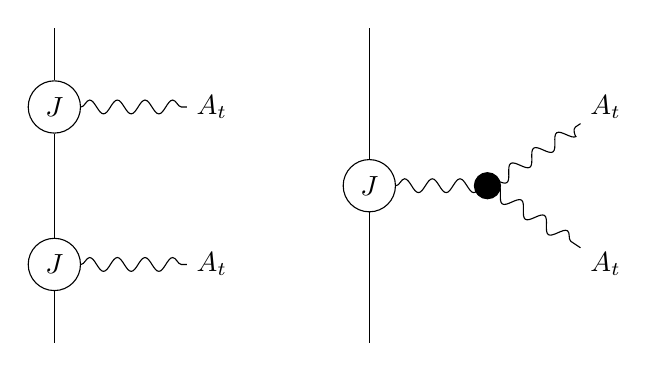
\begin{tikzpicture}
	\begin{scope}
		\node[circle, draw] (J1) at (0,1) {$J$};
		\node[circle, draw] (J2) at (0,-1) {$J$};
		\node (A1) at (2,1)  {$A_{t}$};
		\node (A2) at (2,-1)  {$A_{t}$};
		\draw[decorate, decoration={snake}] (J1) --(A1);
		\draw[decorate, decoration={snake}] (J2) --(A2);
		\draw (0,2) -- (J1) --(J2) -- (0,-2); 
	\end{scope}	
	\begin{scope}[shift={(4,0)}];
		\node[circle, draw] (J) at (0,0) {$J$};
		\node (A1) at (3,1)  {$A_{t}$};
		\node (A2) at (3,-1)  {$A_{t}$};
		\node[circle,draw,fill=black, minimum size = 0.2pt]  (V) at (1.5,0) {};  
		\draw[decorate, decoration={snake}] (J) -- (1.5,0) --  (A1);
		\draw[decorate, decoration={snake}] (1.5,0) --(A2);
		\draw (0,2) -- (J)-- (0,-2);
	\end{scope}
	\end{tikzpicture}
	\caption{Cancellation of the gauge anomaly of these two diagrams leads to the equation for the commutation relations involving the currents $J[k]$.
	\label{fig:cancel1}}
\end{figure}

$\bullet$
Next, let's consider the classical commutation relation 
\begin{equation}\label{eqn:rel2}
[J_a [k] , K_b [\ell]] = f_{ab}^c K_{c} [k+\ell]
\end{equation}

The BRST variation of the term \brian{write path integral above} in the path integral vanishes provided
\[
\int_t \sum_k \frac1{k!} \partial_z^k \left(f_{bc}^a \fc^b(t) B^c_t (t) \right) K_a[k] (t) = \int_t \sum_{\ell,m} \frac1{\ell!} \frac1{m!} \partial^\ell \fc^d (t) \partial^m B^e (t) [J_d (t), K_e(t)]  .
\] 
To obtain the commutation relation \eqref{eqn:rel2}, one sets 
\begin{align*}
B_t & = \ft_b z^{m} \delta_{t=0} \\
\fc & = \ft_a z^\ell .
\end{align*}

This commutation relation is equivalent to the cancellation of the gauge variation of the tree-level Feynman diagrams in Figure~\ref{fig:cancel2}.

\begin{figure}
	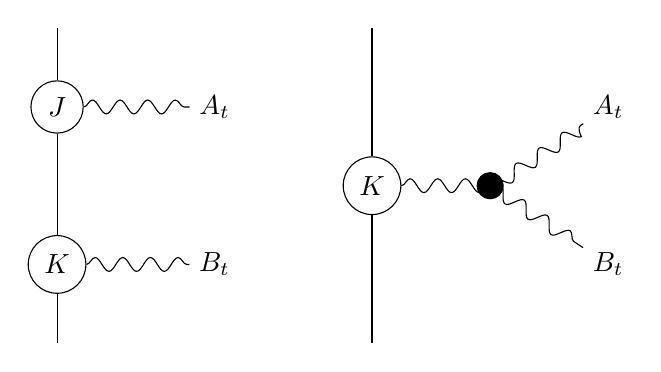
\begin{tikzpicture}
	\begin{scope}
		\node[circle, draw] (J1) at (0,1) {$J$};
		\node[circle, draw] (J2) at (0,-1) {$K$};
		\node (A1) at (2,1)  {$A_{t}$};
		\node (A2) at (2,-1)  {$B_{t}$};
		\draw[decorate, decoration={snake}] (J1) --(A1);
		\draw[decorate, decoration={snake}] (J2) --(A2);
		\draw (0,2) -- (J1) --(J2) -- (0,-2); 
	\end{scope}	
	\begin{scope}[shift={(4,0)}];
		\node[circle, draw] (J) at (0,0) {$K$};
		\node (A1) at (3,1)  {$A_{t}$};
		\node (A2) at (3,-1)  {$B_{t}$};
		\node[circle,draw,fill=black, minimum size = 0.2pt]  (V) at (1.5,0) {};  
		\draw[decorate, decoration={snake}] (J) -- (1.5,0) --  (A1);
		\draw[decorate, decoration={snake}] (1.5,0) --(A2);
		\draw (0,2) -- (J)-- (0,-2);
	\end{scope}
	\end{tikzpicture}
	\caption{Cancellation of the gauge anomaly of these two diagrams leads to the equation for the commutation relations involving $J[k]$ and $K[\ell]$.
	\label{fig:cancel2}}
\end{figure}

\subsection*{Quantum corrections}

We now turn to quantum corrections to the Koszul dual algebra.

The second diagram in Figure \ref{fig:cancel3} has a gauge anomaly.
We will show that this gauge anomaly is proportional to 
\[
\hbar \int_{\RR \times \{z=0\}} \partial_z \fc^a \kappa^{bc} f_{ab}^d J_{c} K_{d} + \cdots .
\]
The ellipses denote similar terms present in the anomaly which involve a higher number of holomorphic $z$-derivatives 

The second diagram in Figure \ref{fig:cancel4} also has a gauge anomaly.
We will show that this gauge anomaly is proportional to 
\[
\hbar \int_{\RR \times \{z=0\}} \partial_z \fc^a \kappa^{bc} f_{ab}^d K_{c} K_{d} + \cdots .
\]


\begin{figure}
	\begin{tikzpicture}
	\begin{scope}
		\node[circle, draw] (J) at (0,0) {$J$};
		%\node[circle, draw] (J2) at (0,-1) {$K$};
		\node (A) at (2,0)  {$A_{t}$};
		%\node (A2) at (2,-1)  {$B_{t}$};
		\draw[decorate, decoration={snake}] (J) --(A);
		%\draw[decorate, decoration={snake}] (J2) --(A2);
		\draw (0,2) -- (J) -- (0,-2); 
	\end{scope}	
	\begin{scope}[shift={(4,0)}];
		\node[circle, draw] (K) at (0,1) {$K$};
		\node[circle, draw] (J) at (0,-1) {$J$};
		\node (A) at (3,0)  {$A_{t}$};
		%\node (A2) at (3,-1)  {$B_{t}$};
		\node[circle,draw,fill=black, minimum size = 0.2pt]  (V) at (1.5,0) {};  
		\draw[decorate, decoration={snake}] (J) -- (1.5,0);
		\draw[decorate, decoration={snake}] (1.5,0) --(A);
		\draw[decorate, decoration={snake}] (K) -- (1.5,0);
		\draw (0,-2) -- (J) -- (K) -- (0,2);
	\end{scope}
	\end{tikzpicture}
	\caption{Cancellation of the gauge anomaly of these two diagrams leads to the $\hbar$-linear correction to the differential $\d J[k]$.
	\label{fig:cancel3}}
\end{figure}

\begin{figure}
	\begin{tikzpicture}
	\begin{scope}
		\node[circle, draw] (K) at (0,0) {$K$};
		%\node[circle, draw] (J2) at (0,-1) {$K$};
		\node (B) at (2,0)  {$B_{t}$};
		%\node (A2) at (2,-1)  {$B_{t}$};
		\draw[decorate, decoration={snake}] (K) --(B);
		%\draw[decorate, decoration={snake}] (J2) --(A2);
		\draw (0,2) -- (K) -- (0,-2); 
	\end{scope}	
	\begin{scope}[shift={(4,0)}];
		\node[circle, draw] (K1) at (0,1) {$K$};
		\node[circle, draw] (K2) at (0,-1) {$K$};
		\node (B) at (3,0)  {$B_{t}$};
		%\node (A2) at (3,-1)  {$B_{t}$};
		\node[circle,draw,fill=black, minimum size = 0.2pt]  (V) at (1.5,0) {};  
		\draw[decorate, decoration={snake}] (K1) -- (1.5,0);
		\draw[decorate, decoration={snake}] (1.5,0) --(B);
		\draw[decorate, decoration={snake}] (K2) -- (1.5,0);
		\draw (0,-2) -- (K2) -- (K1) -- (0,2);
	\end{scope}
	\end{tikzpicture}
	\caption{Cancellation of the gauge anomaly of these two diagrams leads to the $\hbar$-linear correction to the differential $\d K[k]$.
	\label{fig:cancel4}}
\end{figure}

\natalie{computation needs to be completed}


%Two steps:
%\begin{itemize}
%\item There is a relation in the algebra of local operators of the form
%\[
%[B^b, B^c] = \hbar f^{bc}_a \partial_z B^a + O(\hbar^2)  .
%\]
%This gives rise to a term in the differential on the Koszul dual algebra of the form
%\[
%\d (z \ep \ft_a) = \hbar  f^{bc}_a (\ep \ft_b) \otimes (\ep \ft_c) + O(\hbar^2) .
%\]
%\item There is a relation in the algebra of local operators of the form
%\[
%[B^b, \fc^c] = \hbar f^{bc}_a \partial_z \fc^a + O(\hbar^2) .
%\]
%This gives rise to a term in the differential on the Koszul dual algebra of the form
%\[
%\d (z \ft_a) = \hbar  f^{bc}_a (\ep \ft_b) \otimes (\ft_c) + O(\hbar^2) .
%\]
%\brian{do I need to symmetrize?}
%\end{itemize}
\section{Higher dimensional defects} 
%A few words about En algebras

%higher dimensional topological defects. PSM in 3dCS. 
%Kapustin--Salina.
%Check refs by Mnev et al on BV-BFV?

\section{Conclusions and further directions}

\natalie{remark on the transverse boundary condition computation of the free field example, explain that the two pictures of KD connect (lines and boundaries), cite Tudor's String-Math talk, remark on it as future work}

\natalie{some basic comments on modules (lines ending on surface defects), cite Davide/s paper with Miro on OPEs of lines/surfaces in twisted M-theory}

\natalie{we may want to make a few remarks about higher dimensional topological defects and En algebras here, rather than have a separate section}

\natalie{line defects of disorder type: cite Kevin/Davide/Junya}

\natalie{Koszul duality for VOAs, applications to twisted holography}



\printbibliography

\end{document}